\documentclass[11pt]{caltech_thesis} % font size must be changed in the caltech_thesis.cls file. 
% [11pt] has no effect here
\usepackage[hyphens]{url}
\usepackage{lipsum}
\usepackage{graphicx}
\usepackage{todonotes}
\usepackage[utf8]{inputenc}
\usepackage[T1]{fontenc}
\usepackage{mathpazo}
\usepackage[numbers,sort&compress]{natbib}
\usepackage{csquotes}
\usepackage{bibunits}
\usepackage{enumitem}
\usepackage{amsmath}
\usepackage{longtable}
\usepackage{xcolor} 
\usepackage{indentfirst} 
\usepackage{upgreek} % for non-italic greek letters (units)
\usepackage[outputdir=../]{minted} % for code highlighting
\definecolor{CaltechOrange}{HTML}{FF6C0C}
\definecolor{midnightblue}{HTML}{3F3F9E}
\definecolor{darkred}{HTML}{BA1A1A}
\definecolor{extralightgray}{HTML}{F5F5F5}
\usepackage[hidelinks=true,
            colorlinks=true, 
            linkcolor=black,
            urlcolor=CaltechOrange, 
            linkbordercolor=white,
            backref=false,
            pagebackref=false,
            hyperindex=false,
            breaklinks=true,
            bookmarks=false,
            bookmarksopen=false,
            ]{hyperref}
\usepackage[
            backend=biber,natbib,
            % IMPORTANT: load a style suitable for your discipline
            style=ieee
        ]{biblatex}


% added to conform with this issue: https://github.com/jgm/pandoc/issues/4384
% with this, figure width can be changed with {width: 70%}
\makeatletter
\def\maxwidth{\ifdim\Gin@nat@width>\linewidth\linewidth\else\Gin@nat@width\fi}
\def\maxheight{\ifdim\Gin@nat@height>\textheight\textheight\else\Gin@nat@height\fi}
\makeatother
% Scale images if necessary, so that they will not overflow the page
% margins by default, and it is still possible to overwrite the defaults
% using explicit options in \includegraphics[width, height, ...]{}
\setkeys{Gin}{width=\maxwidth,height=\maxheight,keepaspectratio}

\hypersetup{
  colorlinks = true,
  linkcolor = black
}

\makeatletter
\let\@mycite\@cite
\def\@cite#1#2{{\hypersetup{linkcolor=black!60!black}[{#1\if@tempswa , #2\fi}]}}
\makeatother
            
\addbibresource{references_cleaned.bib}
\defaultbibliographystyle{plainnat}
\renewcommand{\bibsection}{\section*{\refname}}
\usepackage{memhfixc}
\linespread{1.5}


\begin{document}

\title{Towards Precise Quantum Measurements with Superconducting
Nanowire Single Photon Detectors}
\author{Andrew Sterling Mueller}
\degreeaward{Doctor of Philosophy in Applied Physics}                 
\university{California Institute of Technology}    
\address{Pasadena, California}                     
\unilogo{caltech.png}                                 
\copyyear{2024}  
\defenddate{November 2023}   
       
\orcid{0000-0002-6598-9732}



\rightsstatement{Some rights reserved. This thesis is distributed under
a Creative Commons Attribution License CC-BY 4.0. All software used in
the analysis and generation of figures is distributed under an MIT
license, and is available on a GitHub repository
\href{https://github.com/sansseriff/phd_thesis}{https://github.com/sansseriff/phd\textunderscore thesis}}

\maketitle[logo]

\begin{acknowledgements}   
    \input{frontmatter/acknowledgements.md}
\end{acknowledgements}

\begin{abstract}
  \input{frontmatter/abstract.md} 
\end{abstract}

\extrachapter{Published Content and Contributions}
\begin{publishedcontent}
\input{frontmatter/published.md}
\end{publishedcontent}

\tableofcontents
\listoffigures
\listoftables
\printnomenclature
\mainmatter

\hypertarget{low-dark-count-rate-detection}{%
\chapter{Low Dark Count Rate
Detection}\label{low-dark-count-rate-detection}}

The work described in this chapter culminated in the research paper:
Andrew S. Mueller, Boris Korzh, Marcus Runyan, Emma E. Wollman, Andrew
D. Beyer, Jason P. Allmaras, Angel E. Velasco, Ioana Craiciu, Bruce
Bumble, Ryan M. Briggs, Lautaro Narvaez, Cristián Peña, Maria Spiropulu,
and Matthew D. Shaw, ``Free-space coupled superconducting nanowire
single-photon detector with low dark counts,''
\href{https://opg.optica.org/optica/fulltext.cfm?uri=optica-8-12-1586\&id=465726}{Optica
8, 1586-1587 (2021)}

Boriz Korzh provided extensive assistance during ideation, construction,
testing, and copyediting phases of the experiment. Bruce Bumble designed
the elevated 0.8 K stage and innovated translation system using flexible
carbon fiber rods. Jason Trevor provided technical assistance with the
implementation of a nitrogen flow bag. Sahil Patel assisted with editing
the manuscript.

\hypertarget{abstract}{%
\section{Abstract}\label{abstract}}

\emph{A free-space coupled superconducting nanowire single photon
detector with high efficiency at 1550 nm, sub-0.1 Hz dark count rate,
and sub-15 ps timing jitter is demonstrated.}

\hypertarget{background}{%
\subsubsection{Background}\label{background}}

Superconducting nanowire single photon detectors are high sensitive
devices. Any stray photons from a laboratory environment can make their
way into these devices and produce a detection. These detections are
commonly called dark counts or false counts. Dark counts can be present
in any situation where the detector is coupled to some experiment or
apparatus outside the cryogenic environment. This coupling may be
through windows inside the cryostat housing and radiations shields, or
through optical fibers that carry single-mode signals directly to
detectors.

Visible, near-infrared, and mid-infrared photons are often the main
sources of dark counts, because they are ubiquitous in a laboratory
environment and are transmitted through common types of fibers and
windows. Assuming visible light can be blocked from entering the
detector system, the blackbody emission of the room temperature
laboratory environment presents is the primary source of dark counts.
The spectrum of blackbody photons, defined by Planck's law, is peaked at
about \(10~\mathrm{\upmu m}\), though it can contribute dark counts at
significant rates up through near-infrared wavelengths.

Without filtering in fiber or free space, dark counts from blackbody
emission will overload most SNSPDs and overpower the extremely faint
signal of interest.

\hypertarget{introduction}{%
\section{Introduction}\label{introduction}}

Time-resolved photon detection with low dark counts is a vital
technology in fields such as quantum information processing, classical
communication, quantum communication, and laser ranging. Increasingly,
research in these fields employs superconducting nanowire single photon
detectors (SNSPDs), which have been demonstrated with system detection
efficiency (\(\eta\)) of more than 90\% \autocite{Reddy2020}, timing
jitter (\(\Delta t\)) as low as 2.6 ps \autocite{Korzh2020} and
intrinsic dark count rates (\(D\)) in the milli- to micro-hertz range
\autocite{Hochberg2019}. However, quantum communication applications
require detection systems with performance optimized across all three
metrics simultaneously. The dimensionless figure of merit \(H\)
specifies this application-specific performance as
\(H = \frac{\eta}{(\Delta t D)}\) \autocite{Hadfield2009}.

Here, we focus on lowering the Dark Count Rate (DCR) of a telecom-band
SNSPD system by filtering thermal photons, without sacrificing
efficiency or jitter. We demonstrate a free-space coupled SNSPD with
sub-0.1 Hz DCR, 14 ps timing jitter, and 72\% total system detection
efficiency (SDE) by using a differential single-pixel SNSPD
\autocite{Colangelo2021} to image a single-mode fiber through an
optimized free-space filter stack.

The highest system detection efficiencies have been achieved using
self-aligned fiber coupling where dark counts can be reduced using
cryogenic fiber looping \autocite{Cohen2015} or spliced narrow-band
filters \autocite{Boaron2018secure}. But it is difficult to achieve
strong filtering without losses at the target wavelength. Low-loss,
high-rejection filters are typically available as free-space components,
so some of the highest reported H-values were achieved with cryogenic,
fiber to free-space to fiber coupling, but exhibit an SDE of only a few
percent \autocite{Shibata2015}. The filtering method presented here
takes advantage of commercially-available filters, achieves a high
free-space coupling efficiency using a cryogenic lens, and is compatible
with both fiber and free-space optical inputs.

In this work, a single mode fiber is imaged onto the detector using two
f = 18.75 mm lenses. One lens collimates light from an optical fiber
face outside the cryostat (Photon Spot), and the other focuses light
onto the detector inside \autocite{Bellei:16}. In the collimated region
between, the beam passes though a series of short-pass filters and one
band-pass filter mounted at 4 K (Fig. \ref{fig:setup}a). One of the
short-pass filters is angled to avoid ghosting effects. The 40 K
radiation shield and outer cryostat housing are fitted with
anti-reflection coated BK7 windows. The filters are spring loaded to
prevent cracking at low temperatures. To minimize effects of stray
light, the interior of the 4 K shield was painted with mid-IR absorbing
paint (Aeroglaze Z306) \autocite{Persky1999}, while gaps between filters
and the windows were covered with metal tape.

The system is based on 1-inch optics, although the f = 18.75 mm lenses
lead to a \(1/e^2\) intensity diameter of about 5 mm in the collimated
region. To reduce the larger-than-required numerical aperture of the
system, painted 8 mm apertures (Acktar Spectral Black) were added in the
collimated region. These are large enough to allow minor alignment
adjustments --- by translating the exterior collimating lens --- without
vignetting.

\hypertarget{fig:dcrmin_data}{%
\begin{figure}
\centering
\includegraphics{chapter_01/figs_01/DataFigure_6.pdf}
\caption[{Low Dark Count Rate Project Results.}]{\textbf{Low Dark Count
Rate Project Results} a) Simulated photon flux at various temperatures
with and without the 1550 nm bandpass filter (BP). b) Normalized photon
count rate (PCR) and jitter measurements c) DCR, and calculated figure
of merit \(H\) versus bias current for both fiber-coupled and free space
coupled configurations.}
\label{fig:dcrmin_data}
\end{figure}
}

We use four custom cryogenic short-pass filters, with pass-bands below
\(1.6 \ \mathrm{\upmu m}\) and \(1.9 \ \mathrm{\upmu m}\) (Andover
Corp.), both with transmission at 1550 nm of 98.8 ± 0.3\%. They reject
wavelengths shorter than \(3 \ \mathrm{\upmu m}\) through reflective
optical coatings, and attenuate longer wavelengths through material
absorption in the 12.7 mm-thick N-BK7 glass substrate. While the
bandpass filter (FWHM = 7 nm) was found to blue-shift by about 2 nm at
cryogenic temperatures, the passband was wide enough such that
significant attenuation was not observed at the original target
wavelength of 1550 nm. This filter is also sufficiently wide to avoid
Fourier-limited broadening of ultra-short laser pulses.

The filtering of the optical stack was modeled by assuming a black-body
emitter at 298 K and a field of view defined by the 18.75 mm focal
length of the cryogenic lens and the 8 mm diameter of the apertures. The
resulting spectrum was multiplied by the transmission of the filters
(Fig. \ref{fig:setup}b) and detector optical stack (Fig.
\ref{fig:setup}c). The model showed that two each of the
\(1.6 \ \mathrm{\upmu m}\) and \(1.9 \ \mathrm{\upmu m}\) short pass
filters were necessary to suppress mid-infrared light to where it was no
longer the dominant source of dark counts. With the inclusion of the
four shortpass filters, the dominant source of dark counts is the
spectral region near 1550 nm as shown in Fig. \ref{fig:false-color}a,
which also illustrates the effect of the bandpass filter. Also evident
in Fig. \ref{fig:false-color}a is the strong dependence of DCR on the
temperature of the final surface outside the cryostat emitting thermal
radiation. This motivated the exterior cooling apparatus shown at the
bottom of Fig. \ref{fig:setup}a. The bulkhead holding the fiber
connector is cooled to around -2\(^\circ\)C using a Peltier element and
liquid cooling block. This addition reduced the system DCR from 0.4 Hz
to below 0.1 Hz. While dark counts from multiple spatial modes are
present in this system --- modes that would not be present in a purely
fiber based approach --- the external cooling technique works to
minimize their effect.

This work used a low-jitter, differential SNSPD \cite{Colangelo2021},
with an active area of \(22 \times 15 \ \mathrm{\upmu m}\), formed by a
meander of 100 nm-wide and 5-nm-thick niobium nitride (NbN) nanowires on
a 500 nm pitch. A more conventional single-ended readout SNSPD of
similar area would also achieve low DCR in this coupling system, but
would likely achieve a lower performance metric \(H\) from
correspondingly higher jitter. The nanowire is embedded in an
efficiency-enhancing optical stack made of alternating layers of
TiO\(_2\) and SiO\(_2\) and a gold mirror layer. As shown in Fig.
\ref{fig:false-color}b and c, when fiber coupled (without any
fiber-based filtering methods applied), this detector achieved a
saturated SDE of \(84\% \pm 4.4 \%\) and a DCR of 20 Hz at a bias
current of \(16\ \mathrm{\upmu A}\).

~~~~~ As also shown in Fig. \ref{fig:false-color}b, the free-space
coupling system achieves up to \(72 \% \pm 3.7 \%\) SDE as measured from
the fiber outside the cryostat. The reduction in efficiency is likely
due to surface reflections in the free-space optics, and potential
misalignment in the optical baffles. The minimum DCR (Fig.
\ref{fig:false-color}c) at \(72 \%\) SDE is about 0.1 Hz, with a bias
current of 16 \(\mathrm{\upmu A}\). These metrics, with the jitter
measurements shown in Fig. \ref{fig:false-color}b, give a maximum H
value of \(5 \times 10^{11}\) (Fig. \ref{fig:false-color}c). Values as
high as \(1.8 \times 10^{12}\) have been reported before, but at 1.5\%
system detection efficiency \cite{Shibata2015}. Our system shows a low
DCR can be achieved without severe reduction of SDE or usable target
wavelength bandwidth. This is paramount for the future of terrestrial
and space-to-ground quantum communication, since it increases success
rate with finite statistics \cite{Boaron2018secure}. The same techniques
can be applied to emerging SNSPD applications at longer wavelengths,
such as laser ranging \cite{Taylor2019}, where fiber filtering is
impractical. Beyond single-mode applications, our work paves the way to
scalable, low-DCR, multi-mode coupling to SNSPD arrays
\cite{Wollman2019}.

\hypertarget{fig:custom_figure}{%
\begin{figure}
\centering
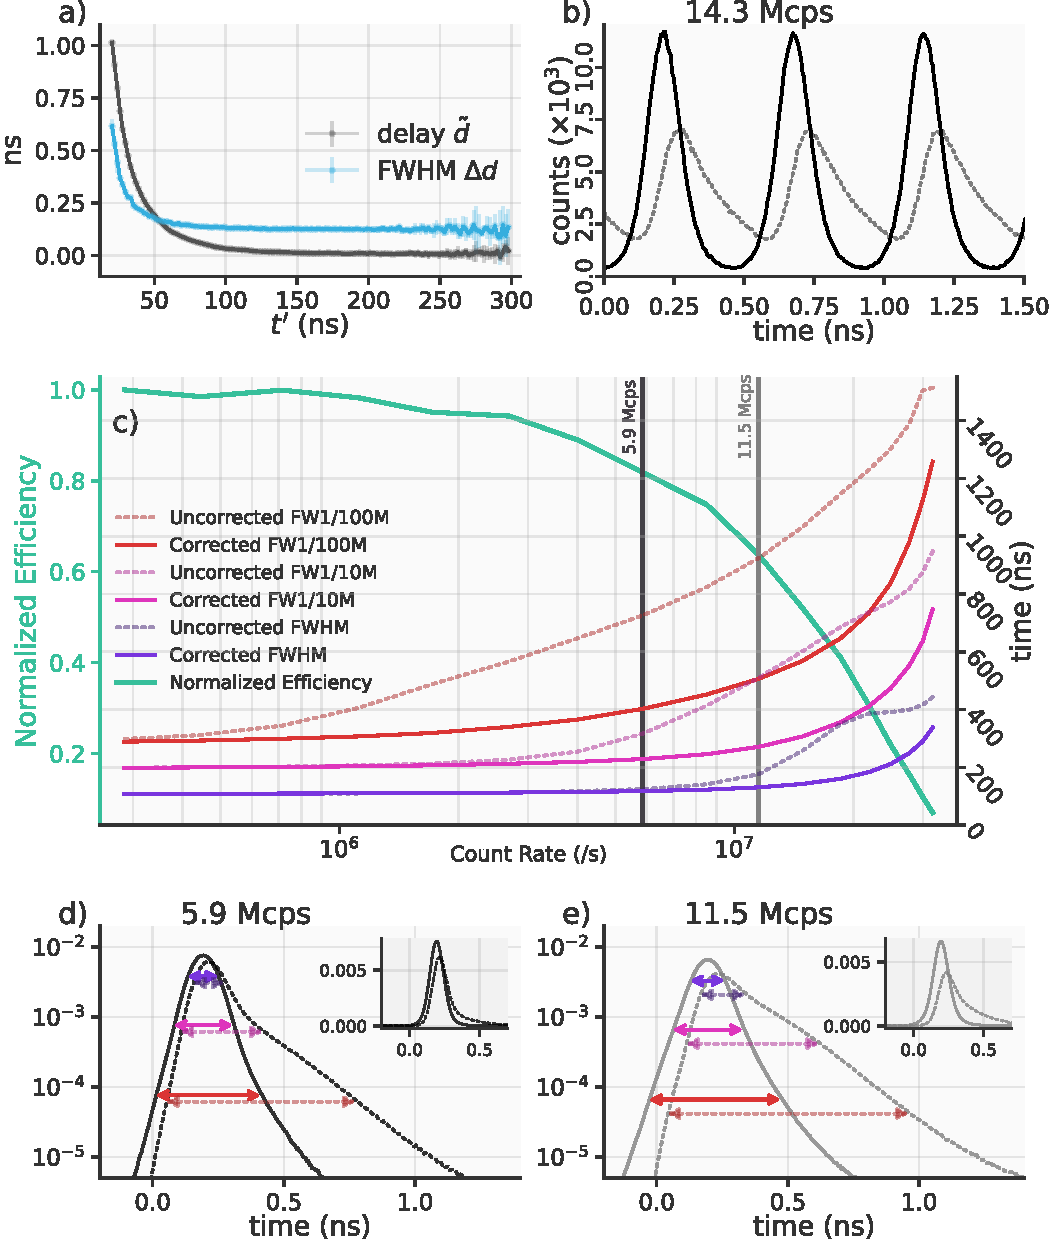
\includegraphics[width=0.7\textwidth,height=\textheight]{chapter_01/figs_01/Figure_Data_Sept_2022_light.pdf}
\caption[{A jitterate data figure.}]{\textbf{Figure Title.} And I think
the rest of this is the caption with (A), (B), and (C) callouts}
\label{fig:custom_figure}
\end{figure}
}

Finally, here's a png figure for testing

\hypertarget{fig:test_png_figure}{%
\begin{figure}
\centering
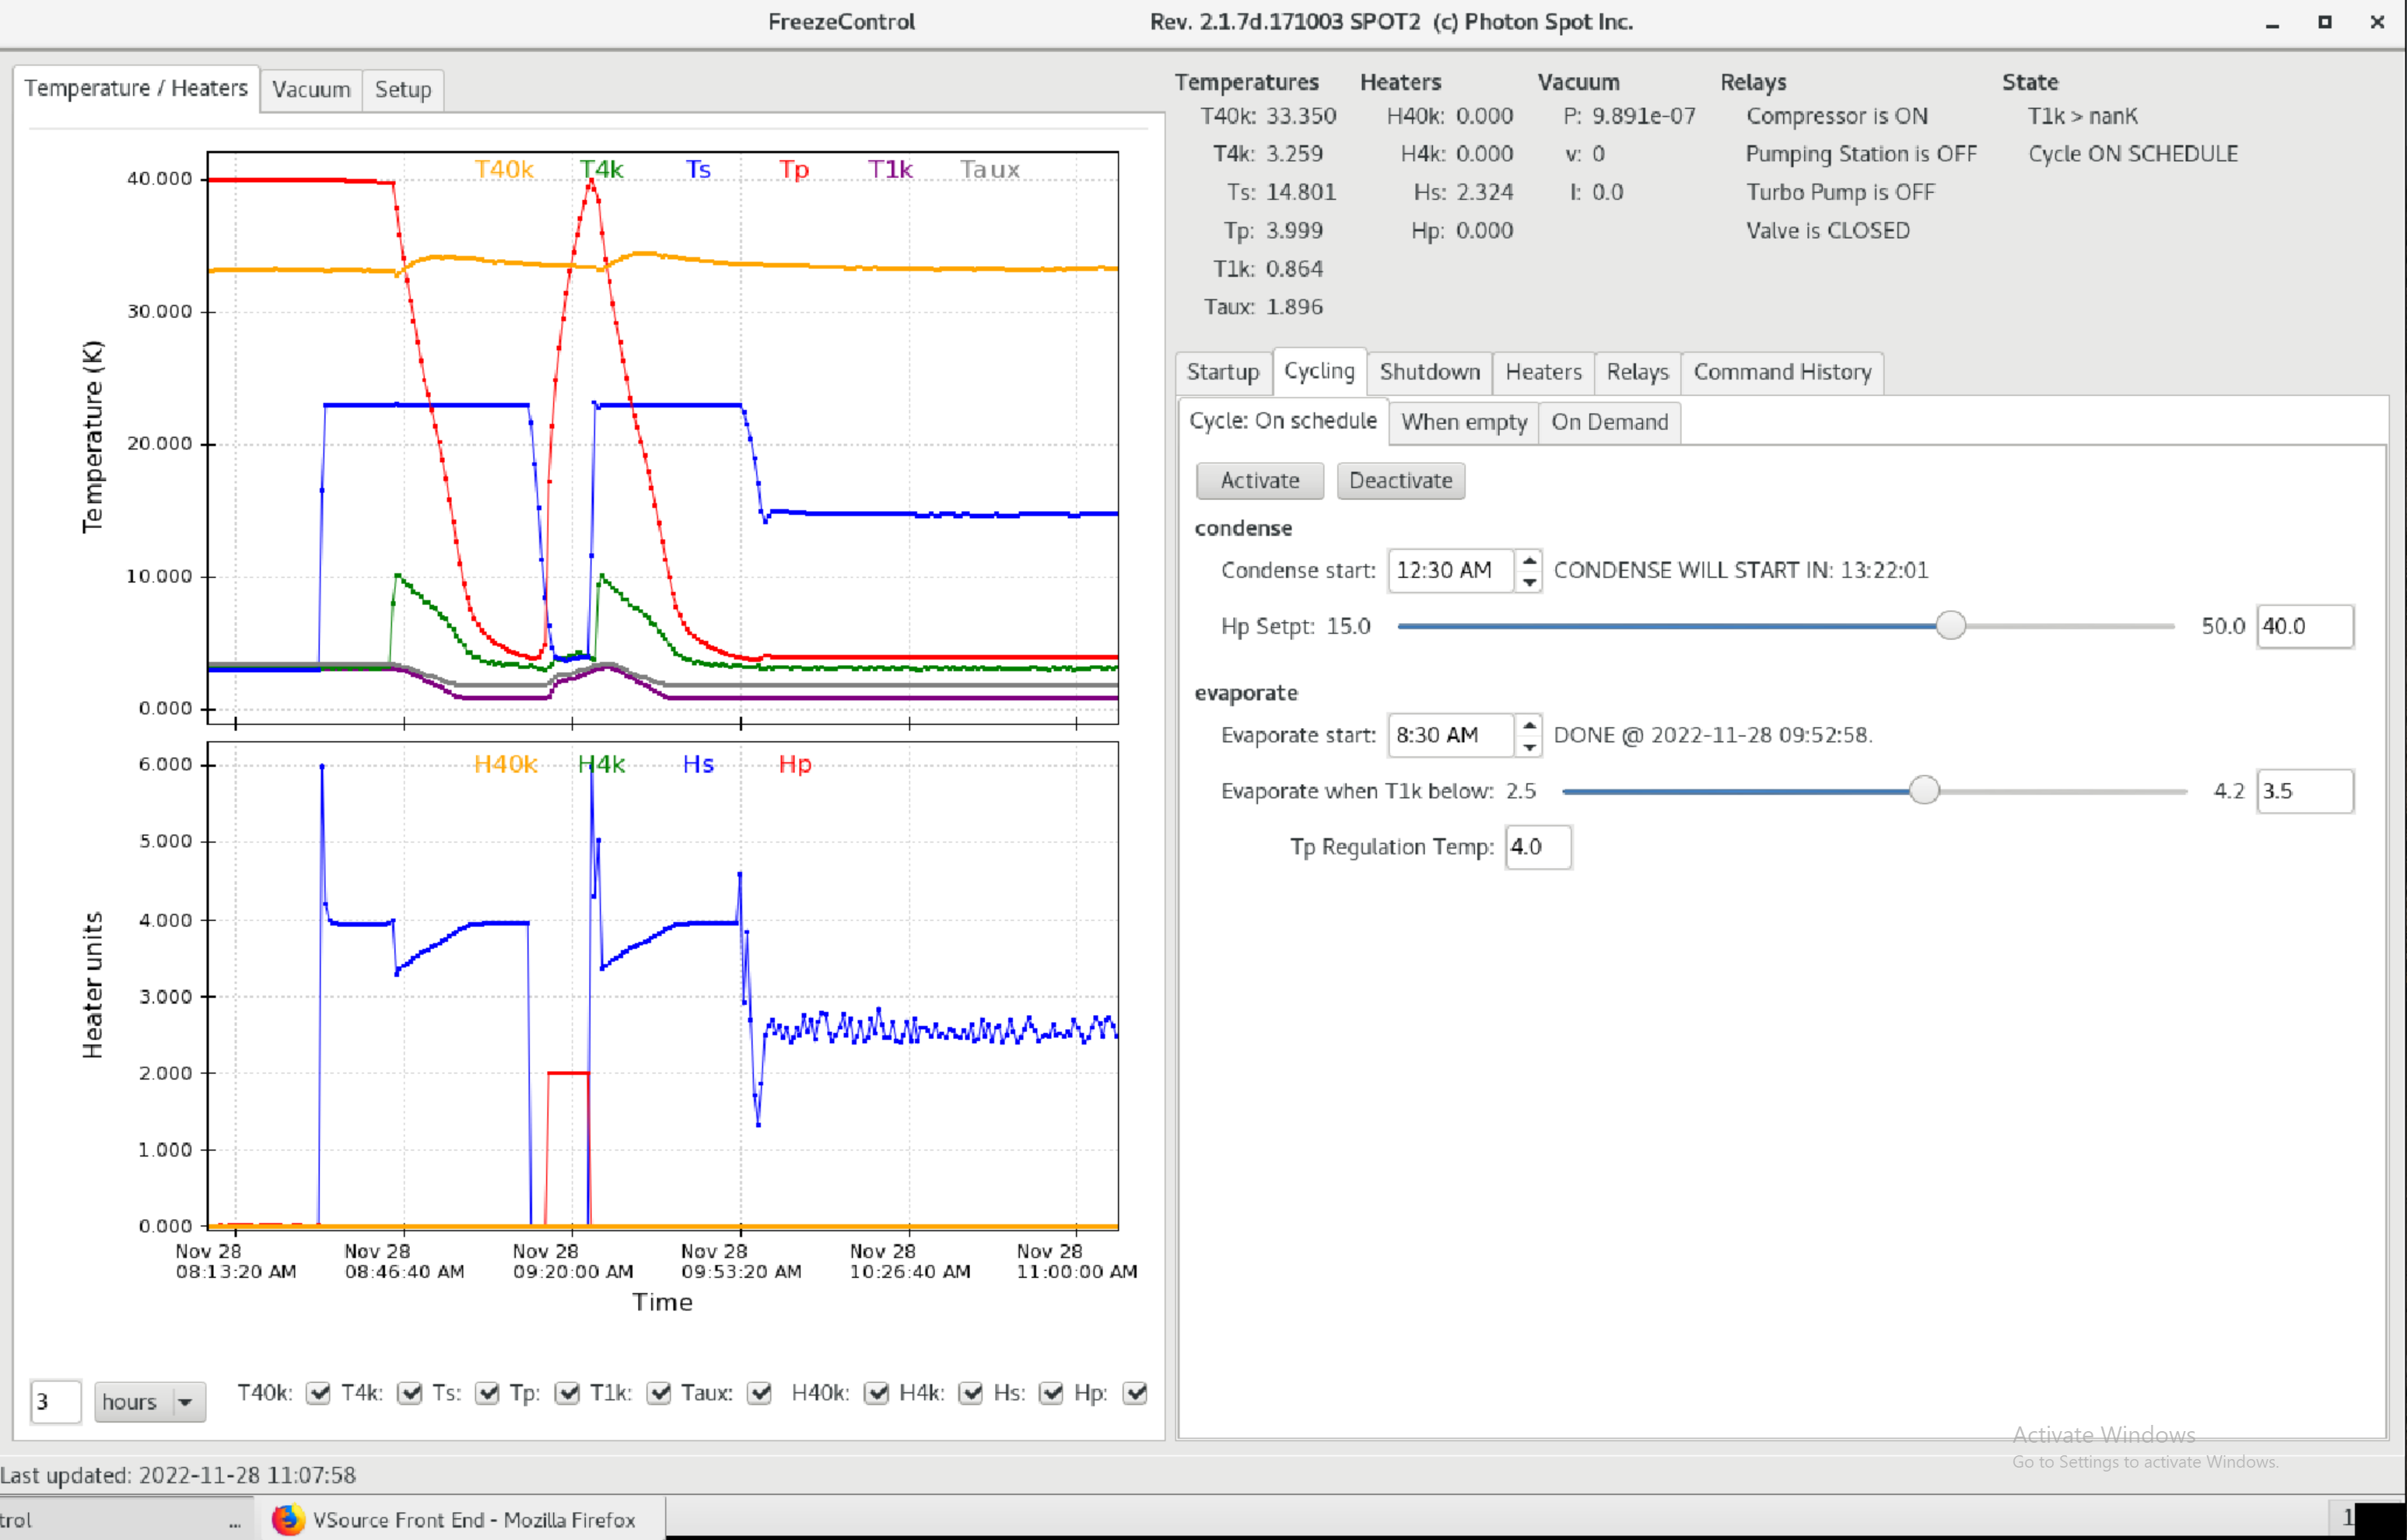
\includegraphics[width=0.7\textwidth,height=\textheight]{chapter_01/figs_01/fridge.png}
\caption[{A png figure.}]{\textbf{A test png figure.} And here is where
I'd put in more information about the png.}
\label{fig:test_png_figure}
\end{figure}
}

Remember there's a lot of optics stuff you got good at, like how to
focus a spot inside the fridge using only optics outside the fridge. How
you used the xyz stage on the fiber for that, and the xy or the mirror.
How you defocused the laser to see the detector when you were using the
narroband filter.

\hypertarget{time-walk-and-jitter-correction}{%
\chapter{Time Walk and Jitter
Correction}\label{time-walk-and-jitter-correction}}

\hypertarget{abstract-1}{%
\section{Abstract}\label{abstract-1}}

~~~~~

\hypertarget{introduction-1}{%
\section{Introduction}\label{introduction-1}}

\hypertarget{method}{%
\section{Method}\label{method}}

Method here

\hypertarget{conclusion}{%
\section{Conclusion}\label{conclusion}}

conclusion here

\hypertarget{the-peacoq-detector-and-higher-order-correction-methods}{%
\section{The Peacoq Detector, and Higher Order Correction
Methods}\label{the-peacoq-detector-and-higher-order-correction-methods}}

Peacoq data and stuff here

\hypertarget{outlook}{%
\section{Outlook}\label{outlook}}

outlook discussion here

Photon number resolution is an emerging capability of advanced
Superconducting Nanowire Single Photon Detectors. If leveraged to it's
full potential, PNR capability can have a profound impact on the
usefulness of SNSPDs is certain quantum applications including linear
optical quantum computing, quantum networks, and quantum sensing.
Discrimination of not just the number of photons in an optical pulse but
also pulse arrival time with high accuracy is an open problem,
complicated by the nuanced way in which these two degrees of freedom are
intertwined in the response function of these detectors. In this work we
put a differential readout SNSPD to the ultimate test. We test it's
capabilities in a Pulse Position Modulation experiment whereby data is
sent in the arrival time of optical pulses derived from a 20~GHz optical
clock. We show the detector is capable of discriminating the arrival
time of photons to 50~ps wide bins with high accuracy while
simultaneously providing photon number information about the impinging
optical pulses. We find that a careful statistical analysis of the PNR
response is necessary to back-out a precise measurement of pulse arrival
time.

\hypertarget{introduction-2}{%
\chapter{Introduction}\label{introduction-2}}

\textcolor{darkred}{ The following is very rough, taken from years ago
when I first started writing the manuscript }

This study aimed to evaluate the feasibility of transmitting high
clock-rate pulse position modulated (PPM) data using a mode-locked laser
and receiving it with a low jitter superconducting nanowire
single-photon detector (SNSPD). The investigation was driven by recent
advancements in NbN SNSPDs, which have achieved a jitter as low as 50 ps
at the FW(1/100)M level, enabling the demonstration of PPM with 50 ps
slot widths and a 20 GHz clock. The aim was to increase the data rate by
a factor of 10, from 2 GHz to 20 GHz, in the next generation of the Deep
Space Optical Communication (DSOC) project.

During the course of this study, the focus shifted towards investigating
the impact of photon number resolution (PNR) on the low jitter detection
of optical pulses. PNR can have an unintended impact on the
demonstration of high-rate PPM, and therefore a thorough study of its
effects was deemed crucial. A novel PNR cancellation technique was
developed and applied to successfully demonstrate high-rate PPM. This
technique is considered essential for future low-jitter applications of
SNSPDs that exhibit photon-number effects.

This study aimed to evaluate the feasibility of transmitting high
clock-rate pulse position modulated (PPM) data using a mode-locked laser
and receiving it with a low jitter superconducting nanowire
single-photon detector (SNSPD). The investigation was driven by recent
advancements in NbN SNSPDs, which have achieved a jitter as low as 50 ps
at the FW(1/100)M level, enabling the demonstration of PPM with 50 ps
slot widths and a 20 GHz clock. The aim was to increase the data rate by
a factor of 10, from 2 GHz to 20 GHz, in the next generation of the Deep
Space Optical Communication (DSOC) project.

During the course of this study, the focus shifted towards investigating
the impact of photon number resolution (PNR) on the low jitter detection
of optical pulses. PNR can have an unintended impact on the
demonstration of high-rate PPM, and therefore a thorough study of its
effects was deemed crucial. A novel PNR cancellation technique was
developed and applied to successfully demonstrate high-rate PPM. This
technique is considered essential for future low-jitter applications of
SNSPDs that exhibit photon-number effects.

\hypertarget{pulse-position-modulation-for-deep-space-communication}{%
\section{Pulse Position Modulation for Deep Space
Communication}\label{pulse-position-modulation-for-deep-space-communication}}

Deep Space Optical Communication has been a growing field of study in
recent years, as researchers look for ways to communicate with
spacecraft that are far away from Earth. In this article, we will focus
on the use of Pulse Position Modulation (PPM) for deep space optical
communication.

While other modulation techniques such as quadrature amplitude
modulation (QAM) have been used in the past, it has been shown that in
the photon-starved regime, PPM is the best approach for sending data.
This is because there is not enough light to measure the phase of the
signal.

PPM relies on sending one optical pulse carrying M bits of information
in one of \(2^M\) possible time slots. For M = 2, this corresponds to
sending an early pulse to represent a 0 bit and a late pulse to
represent a 1 bit.

The main challenge in deep space optical communication is the high loss
and distance that the link must traverse. This limits the communication
from the spacecraft, as it is limited by the power available on the
spacecraft. This means that the communication protocol is limited by the
number of bits that can be sent per unit of energy on the spacecraft,
also known as photon information efficiency or bits per photon.

For large M, PPM achieves high photon information efficiency, allowing
for the saving of power on the spacecraft and the sending of more
information with fewer photons. The existing deep space optical
communication project uses M up to \(2^8 = 256\), meaning that 8 bits of
data are carried in each optical pulse.

In this project, we aimed to demonstrate even higher photon information
efficiency by using M values up to 2048, or 11 bits of data per optical
pulse.

While the use of large M values increases photon information efficiency,
it also decreases the data rate of the system. This is because the
number of time bins needed per optical pulse scales exponentially with
the amount of data in each pulse. Therefore, for a given fixed clock
rate and time bin duration, the data rate decreases dramatically for
higher M values.

Using M values much larger than 11 is unlikely to be practical in future
deep space optical communication systems. However, the data rate of
these systems can be increased linearly by increasing the clock rate or
bin size of the experiment. This is possible with the use of low jitter
detection systems or low jitter superconducting nanowire single-photon
detectors (SNSPDs).

\hypertarget{detector-figure-of-merit}{%
\chapter{Detector Figure of Merit}\label{detector-figure-of-merit}}

The work here highlights the application of low jitter single-photon
detectors for optical communication, which is impactful for deep-space
optical communication as well as classical communication in quantum
networks. Although single-photon counting is well estanblished for
deep-space optical
communication\textasciitilde{}\autocite{Laser,lunar,DSOC} so far it has
not been ulitized in quantum networks, mainly due to the use of SFP
modules and DWDMs. However, with the eachievement of high data rates
recently achieved with photon-counting classical communication, these
approaches can now be seriously considered for quantum networks. The
main driver is would be the deduction of optical power in neighbouring
DWDM channels, which ultimately lowers the Raman scattered photons into
the quantum channel \autocite{EraerdsRaman}
\textcolor{darkred}{Calculate reduction in power from state of the art
SFP modules}

To access the applicability of different detectors, here we compare some
of the recent near infrared detectors.

A useful figure of merit that includes all of the revelant detector
metrics for photon timing was introduced by Bronzi and co-authors
\autocite{Bronzi2016}

\[FoM_T = \frac{\eta  (1 - P_{ap})\Phi_{-3 \text{dB}}}{J} \sqrt{\frac{A}{D}},\]

where \(\eta\) is the single photon detection efficiency,
\(\Phi_{-3 \text{dB}}\) is the photon flux at which the system detection
efficiency drops by 3\textasciitilde dB, \(P_{ap}\) is the afterpulsing
probability, \(J\) is the detector jitter evaluated as the FWHM, \(T_d\)
is the deadtime, \(A\) is the active area and \(D\) is the dark count
rate. Here we have defined the maximum photon flux as the
3\textasciitilde dB point, for ease of standardization.

In this work:

\begin{itemize}
\item
  Efficiency = 0.84
\item
  Afterpulsing = 0 \%
\item
  Jitter = 15 ps
\item
  Deadtime = 30 ns \textcolor{darkred}{measure 3dB flux}
\item
  Area = 330 \(\mu m^2\)
\item
  Dark count rate = 20~Hz
\end{itemize}

\(FoM_T = 7.58 \times 10^{12}\) at 1550 nm.

The deadtime is calculated as the 1/MCR, which is the 3 dB point of the
nominal efficiency. This is only a factor of 3.7 less than the state of
the art visible Silicon SPADs (peak efficiency at 480)
\autocite{Gramuglia2022}

In the future, the performance of the optical communication system could
be improved by using, high count rate SNSPD arrays. Recently published
high-count rate arrays have figures of merit of
\textcolor{darkred}{FoM\_T for Peacoq and Resta2023 results}. This would
result in a proportinal increase in the data rate.
\textcolor{darkred}{FoM\_T for fastest InGaAs/InP gated detector} These
devices are ideal for fiber-based optical communication. In free-space,
the active area is especially important, whithout the use of an adaptive
optics system. \textcolor{darkred}{FoM\_T for DSOC array}

\hypertarget{development-of-a-modulation-source}{%
\section{Development of a modulation
source}\label{development-of-a-modulation-source}}

The communication signal on a spacecraft is generated by utilizing a
Continuous Wave (CW) seed laser that is carved by a fast intensity
modulator. The resulting low-power pulsed signal is then amplified by an
Erbium Doped Fiber Amplifier (EDFA) to increase its transmission power
to Earth. The majority of the power used by the spacecraft for
communication scales with the number of optical pulses due to the EDFA.

In our experiment, the 20 GHz repetition rate was limited by the jitter
of the Single-Photon Detectors (SNSPDs) that we intended to use. These
detectors have a Full Width at Half Maximum (FW(1/100)M) jitter of
approximately 50 ps. To ensure that the response function of the entire
experiment had jitter of around 50 ps FW(1/100)M, we needed to build a
Pulsed Phase Modulation (PPM) source with ultra-short optical pulses.

Carving a CW laser with our system would have introduced excessive
timing uncertainty due to the limited ability of even the fastest
lithium niobate intensity modulators to carve pulses with widths below
20 ps. The added jitter from modulated CW pulses, combined with the
jitter of the detectors, would have exceeded the 20 GHz/50 ps slot width
requirement.

Therefore, we chose to carve pulses from a mode-locked laser. This
approach allows for extremely short pulses in time, with the modulators
responsible for sufficiently reducing any surrounding unwanted pulses.
The temporal width of the modulator pulse response must be extremely
short and able to modulate from `off' to `on' within a time frame of the
order of the 50 ps bin width.

\hypertarget{methods}{%
\chapter{Methods}\label{methods}}

\hypertarget{results}{%
\chapter{Results}\label{results}}

results here

\hypertarget{pulse-position-modulation-and-pnr-resolution}{%
\chapter{Pulse Position Modulation and PNR
Resolution}\label{pulse-position-modulation-and-pnr-resolution}}

A version of this chapter will appear as Optix Express arciel
XXX\ldots{}

\hypertarget{abstract-2}{%
\section{Abstract}\label{abstract-2}}

Photon number resolution is an emerging capability of advanced
Superconducting Nanowire Single Photon Detectors. If leveraged to it's
full potential, PNR capability can have a profound impact on the
usefulness of SNSPDs is certain quantum applications including linear
optical quantum computing, quantum networks, and quantum sensing.
Discrimination of not just the number of photons in an optical pulse but
also pulse arrival time with high accuracy is an open problem,
complicated by the nuanced way in which these two degrees of freedom are
intertwined in the response function of these detectors. In this work we
put a differential readout SNSPD to the ultimate test. We test it's
capabilities in a Pulse Position Modulation experiment whereby data is
sent in the arrival time of optical pulses derived from a 20~GHz optical
clock. We show the detector is capable of discriminating the arrival
time of photons to 50~ps wide bins with high accuracy while
simultaneously providing photon number information about the impinging
optical pulses. We find that a careful statistical analysis of the PNR
response is necessary to back-out a precise measurement of pulse arrival
time.

\hypertarget{introduction-3}{%
\section{Introduction}\label{introduction-3}}

\protect\hypertarget{..ux2fcodeux2ftest_1}{}{}

This study aimed to evaluate the feasibility of transmitting high
clock-rate pulse position modulated (PPM) data using a mode-locked laser
and receiving it with a low jitter superconducting nanowire
single-photon detector (SNSPD). The investigation was driven by recent
advancements in NbN SNSPDs, which have achieved a jitter as low as 50 ps
at the FW(1/100)M level, enabling the demonstration of PPM with 50 ps
slot widths and a 20 GHz clock. The aim was to increase the data rate by
a factor of 10, from 2 GHz to 20 GHz, in the next generation of the Deep
Space Optical Communication (DSOC) project.

During the course of this study, the focus shifted towards investigating
the impact of photon number resolution (PNR) on the low jitter detection
of optical pulses. PNR can have an unintended impact on the
demonstration of high-rate PPM, and therefore a thorough study of its
effects was deemed crucial. A novel PNR cancellation technique was
developed and applied to successfully demonstrate high-rate PPM. This
technique is considered essential for future low-jitter applications of
SNSPDs that exhibit photon-number effects.

This study aimed to evaluate the feasibility of transmitting high
clock-rate pulse position modulated (PPM) data using a mode-locked laser
and receiving it with a low jitter superconducting nanowire
single-photon detector (SNSPD). The investigation was driven by recent
advancements in NbN SNSPDs, which have achieved a jitter as low as 50 ps
at the FW(1/100)M level, enabling the demonstration of PPM with 50 ps
slot widths and a 20 GHz clock. The aim was to increase the data rate by
a factor of 10, from 2 GHz to 20 GHz, in the next generation of the Deep
Space Optical Communication (DSOC) project.

During the course of this study, the focus shifted towards investigating
the impact of photon number resolution (PNR) on the low jitter detection
of optical pulses. PNR can have an unintended impact on the
demonstration of high-rate PPM, and therefore a thorough study of its
effects was deemed crucial. A novel PNR cancellation technique was
developed and applied to successfully demonstrate high-rate PPM. This
technique is considered essential for future low-jitter applications of
SNSPDs that exhibit photon-number effects.

\hypertarget{fig:intro}{%
\begin{figure}
\centering
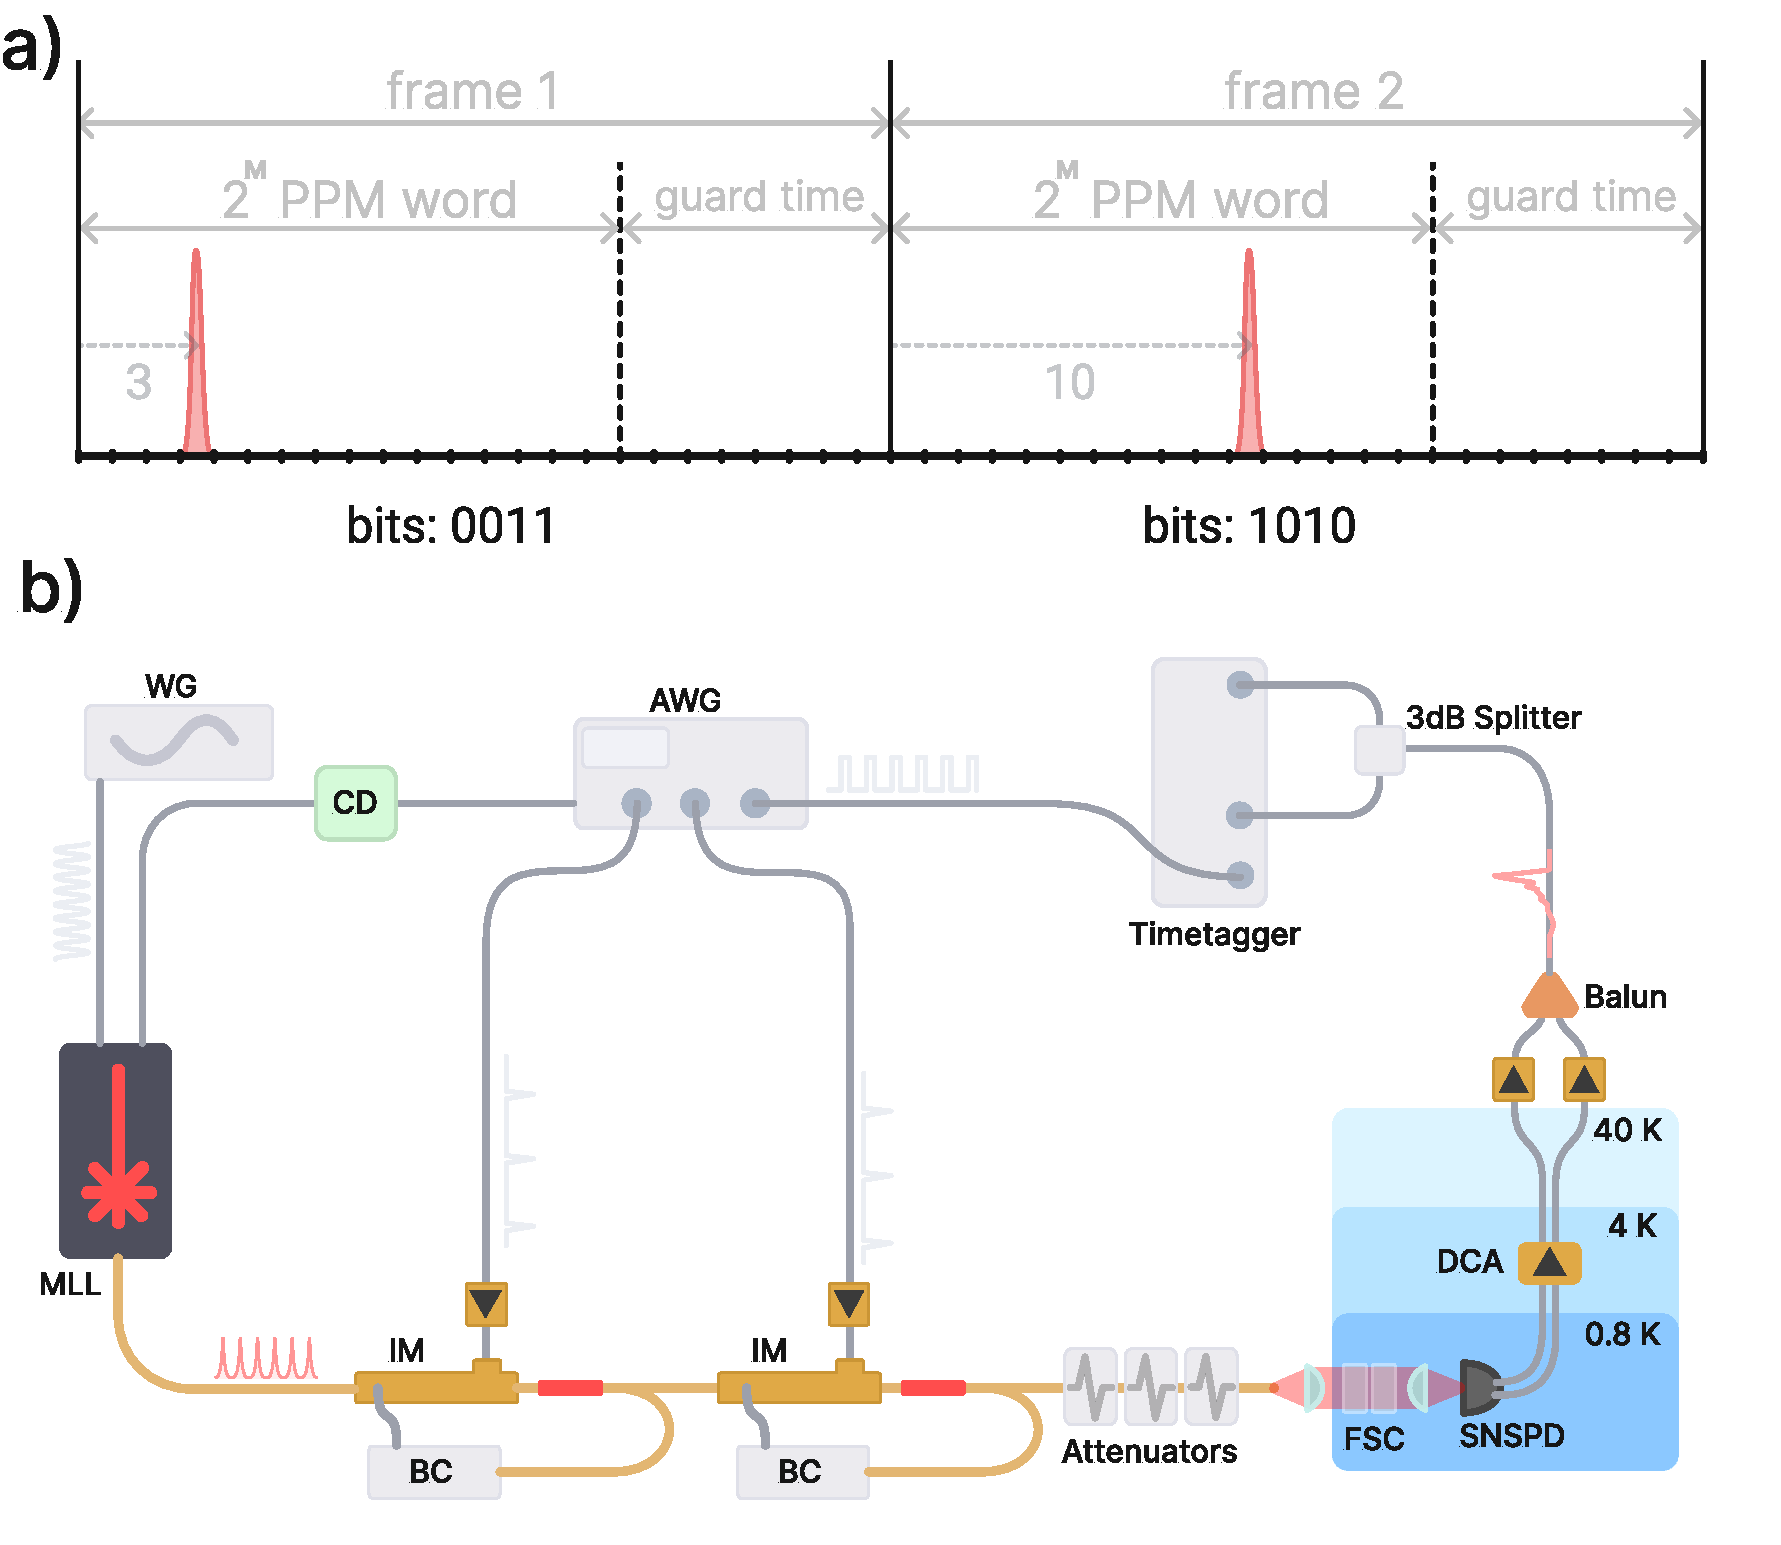
\includegraphics[width=0.8\textwidth,height=\textheight]{chapter_03/figs_03/fig_intro_light.pdf}
\caption[{PPM modulation and experiment setup}]{\textbf{PPM modulation
and experiment setup} a) How bits are transmitted in M=16 PPM
modulation. An optical pulse is transmitted with a clock-referenced
integer delay which encodes 4 bits of data. b) Diagram of the
expiremental setup. WG: wave generator, CD: clock divider board, AWG:
Arbitrary Waveform Generator, MLL: Mode Locked Laser (Pritel UAC), IM:
Intensity Modulator, BC: Bias Controller, FSC: Free Space Coupling
System, DCA: DC Coupled Cryo-amp}
\label{fig:intro}
\end{figure}
}

\hypertarget{pulse-position-modulation-for-deep-space-communication-1}{%
\subsection{Pulse Position Modulation for Deep Space
Communication}\label{pulse-position-modulation-for-deep-space-communication-1}}

Deep Space Optical Communication has been a growing field of study in
recent years, as researchers look for ways to communicate with
spacecraft that are far away from Earth. In this article, we will focus
on the use of Pulse Position Modulation (PPM) for deep space optical
communication.

While other modulation techniques such as quadrature amplitude
modulation (QAM) have been used in the past, it has been shown that in
the photon-starved regime, PPM is the best approach for sending data.
This is because there is not enough light to measure the phase of the
signal.

PPM relies on sending one optical pulse carrying M bits of information
in one of \(2^M\) possible time slots. For M = 2, this corresponds to
sending an early pulse to represent a 0 bit and a late pulse to
represent a 1 bit.

The main challenge in deep space optical communication is the high loss
and distance that the link must traverse. This limits the communication
from the spacecraft, as it is limited by the power available on the
spacecraft. This means that the communication protocol is limited by the
number of bits that can be sent per unit of energy on the spacecraft,
also known as photon information efficiency or bits per photon.

For large M, PPM achieves high photon information efficiency, allowing
for the saving of power on the spacecraft and the sending of more
information with fewer photons. The existing deep space optical
communication project uses M up to \(2^8 = 256\), meaning that 8 bits of
data are carried in each optical pulse.

In this project, we aimed to demonstrate even higher photon information
efficiency by using M values up to 2048, or 11 bits of data per optical
pulse.

While the use of large M values increases photon information efficiency,
it also decreases the data rate of the system. This is because the
number of time bins needed per optical pulse scales exponentially with
the amount of data in each pulse. Therefore, for a given fixed clock
rate and time bin duration, the data rate decreases dramatically for
higher M values.

Using M values much larger than 11 is unlikely to be practical in future
deep space optical communication systems. However, the data rate of
these systems can be increased linearly by increasing the clock rate or
bin size of the experiment. This is possible with the use of low jitter
detection systems or low jitter superconducting nanowire single-photon
detectors (SNSPDs).

\hypertarget{fig:waveform}{%
\begin{figure}
\centering
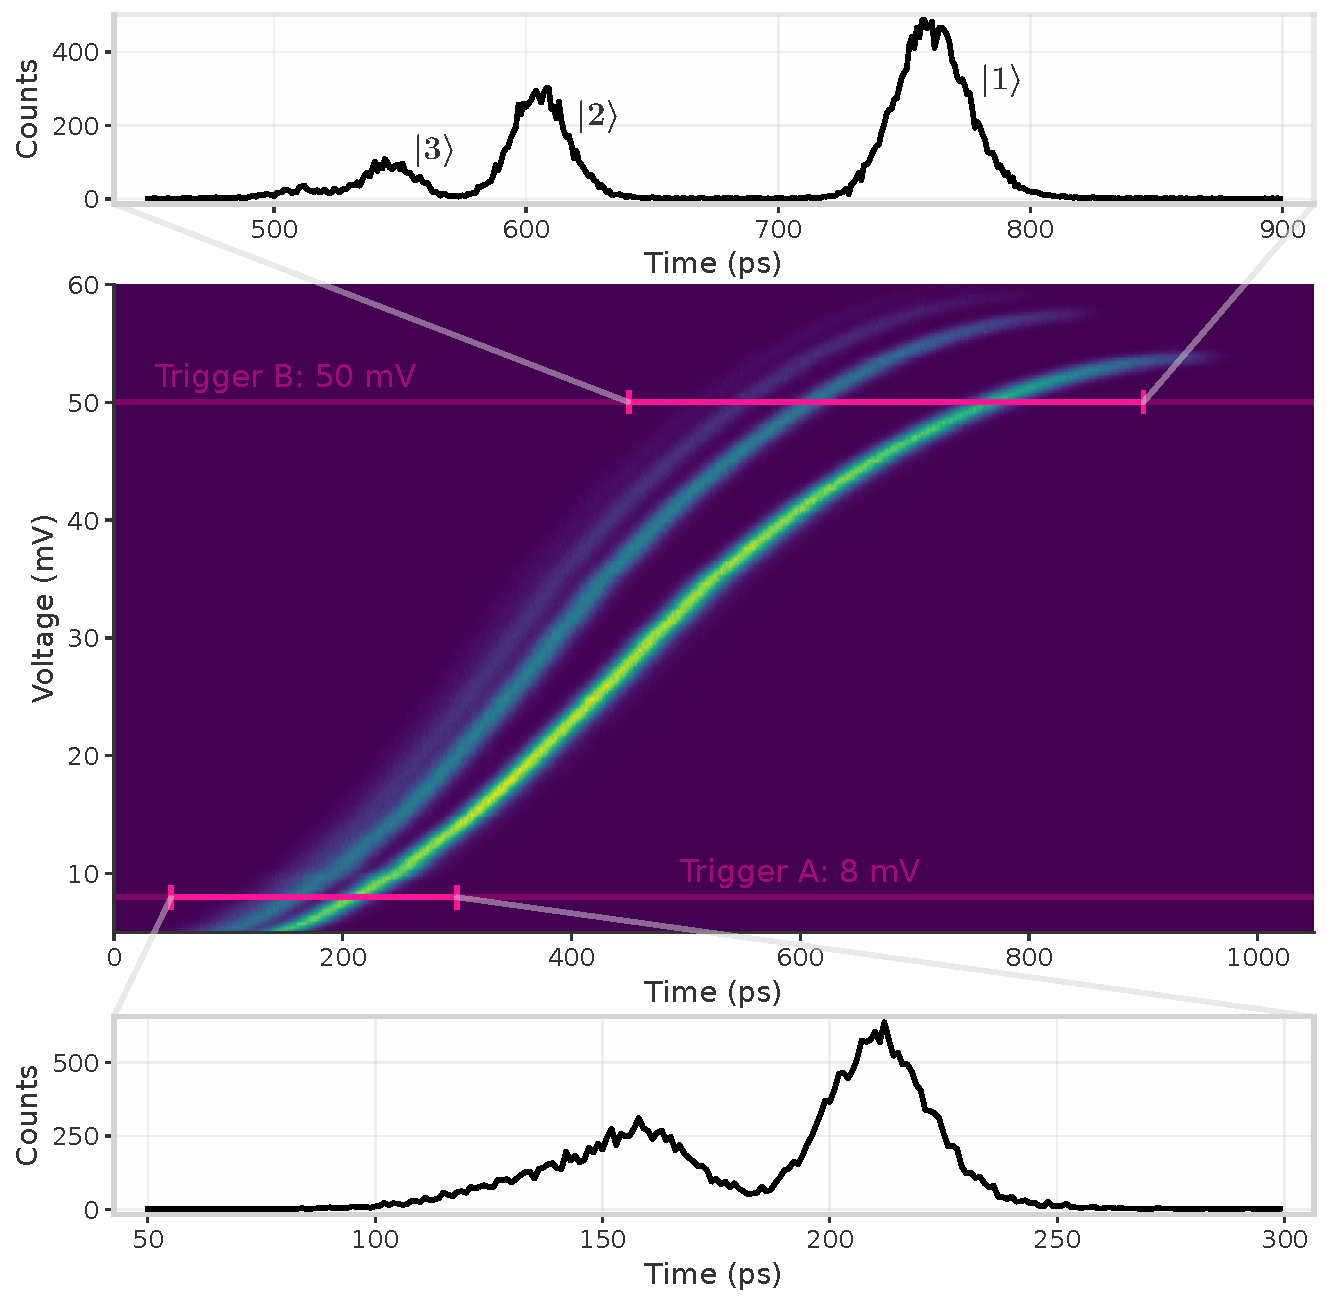
\includegraphics[width=0.8\textwidth,height=\textheight]{chapter_03/figs_03/waveform_light.pdf}
\caption[{PNR-sensitive Pulse Waveform}]{\textbf{PNR-sensitive Pulse
Waveform} The rising edge of the differential SNSPD's RF pulses exibit
variations in height, slew rate, and arrival time due to photon-number
dependent dynamics. The slopes of the 1-photon and 2-photon pulses
significantly differ, and as the photon number increases, the
alterations to the pulse shape become progressively smaller. Trigger
levels A (8~mV) and B (50~mV) were used to extract as much information
about pulse slope and arrival time as possible}
\label{fig:waveform}
\end{figure}
}

\hypertarget{detector-figure-of-merit-1}{%
\section{Detector Figure of Merit}\label{detector-figure-of-merit-1}}

The work here highlights the application of low jitter single-photon
detectors for optical communication, which is impactful for deep-space
optical communication as well as classical communication in quantum
networks. Although single-photon counting is well estanblished for
deep-space optical
communication\textasciitilde{}\cite{Laser lunar, DSOC} so far it has not
been ulitized in quantum networks, mainly due to the use of SFP modules
and DWDMs. However, with the eachievement of high data rates recently
achieved with photon-counting classical communication, these approaches
can now be seriously considered for quantum networks. The main driver is
would be the deduction of optical power in neighbouring DWDM channels,
which ultimately lowers the Raman scattered photons into the quantum
channel \autocite{EraerdsRaman} {Calculate reduction in power from state
of the art SFP modules}

To access the applicability of different detectors, here we compare some
of the recent near infrared detectors.

A useful figure of merit that includes all of the revelant detector
metrics for photon timing was introduced by Bronzi and co-authors
\autocite{Bronzi2016}

\[FoM_T = \frac{\eta  (1 - P_{ap})\Phi_{-3 \text{dB}}}{J} \sqrt{\frac{A}{D}},\]

where \(\eta\) is the single photon detection efficiency,
\(\Phi_{-3 \text{dB}}\) is the photon flux at which the system detection
efficiency drops by 3\textasciitilde dB, \(P_{ap}\) is the afterpulsing
probability, \(J\) is the detector jitter evaluated as the FWHM, \(T_d\)
is the deadtime, \(A\) is the active area and \(D\) is the dark count
rate. Here we have defined the maximum photon flux as the
3\textasciitilde dB point, for ease of standardization.

In this work:

\begin{itemize}
\tightlist
\item
  Efficiency = 0.84
\item
  Afterpulsing = 0 \%
\item
  Jitter = 15 ps
\item
  Deadtime = 30 ns {measure 3dB flux}
\item
  Area = 330 \(\mu m^2\)
\item
  Dark count rate = 20~Hz
\end{itemize}

\(FoM_T = 7.58 \times 10^{12}\) at 1550 nm.

The deadtime is calculated as the 1/MCR, which is the 3 dB point of the
nominal efficiency. This is only a factor of 3.7 less than the state of
the art visible Silicon SPADs (peak efficiency at 480\nm)
\autocite{Gramuglia2022}

In the future, the performance of the optical communication system could
be improved by using, high count rate SNSPD arrays. Recently published
high-count rate arrays have figures of merit of {\(FoM_T\) for Peacoq
and Resta2023 results}. This would result in a proportinal increase in
the data rate. {\(FoM_T\) for fastest InGaAs/InP gated detector} These
devices are ideal for fiber-based optical communication. In free-space,
the active area is especially important, whithout the use of an adaptive
optics system. {\(FoM_T\) for DSOC array}

\hypertarget{development-of-a-modulation-source-1}{%
\subsection{Development of a modulation
source}\label{development-of-a-modulation-source-1}}

The communication signal on a spacecraft is generated by utilizing a
Continuous Wave (CW) seed laser that is carved by a fast intensity
modulator. The resulting low-power pulsed signal is then amplified by an
Erbium Doped Fiber Amplifier (EDFA) to increase its transmission power
to Earth. The majority of the power used by the spacecraft for
communication scales with the number of optical pulses due to the EDFA.

In our experiment, the 20 GHz repetition rate was limited by the jitter
of the Single-Photon Detectors (SNSPDs) that we intended to use. These
detectors have a Full Width at Half Maximum (FW(1/100)M) jitter of
approximately 50 ps. To ensure that the response function of the entire
experiment had jitter of around 50 ps FW(1/100)M, we needed to build a
Pulsed Phase Modulation (PPM) source with ultra-short optical pulses.

Carving a CW laser with our system would have introduced excessive
timing uncertainty due to the limited ability of even the fastest
lithium niobate intensity modulators to carve pulses with widths below
20 ps. The added jitter from modulated CW pulses, combined with the
jitter of the detectors, would have exceeded the 20 GHz/50 ps slot width
requirement.

Therefore, we chose to carve pulses from a mode-locked laser. This
approach allows for extremely short pulses in time, with the modulators
responsible for sufficiently reducing any surrounding unwanted pulses.
The temporal width of the modulator pulse response must be extremely
short and able to modulate from `off' to `on' within a time frame of the
order of the 50 ps bin width.

\hypertarget{methods-1}{%
\section{Methods}\label{methods-1}}

\hypertarget{slope-correction}{%
\subsection{Slope Correction}\label{slope-correction}}

\hypertarget{fig:slope-correction}{%
\begin{figure}
\centering
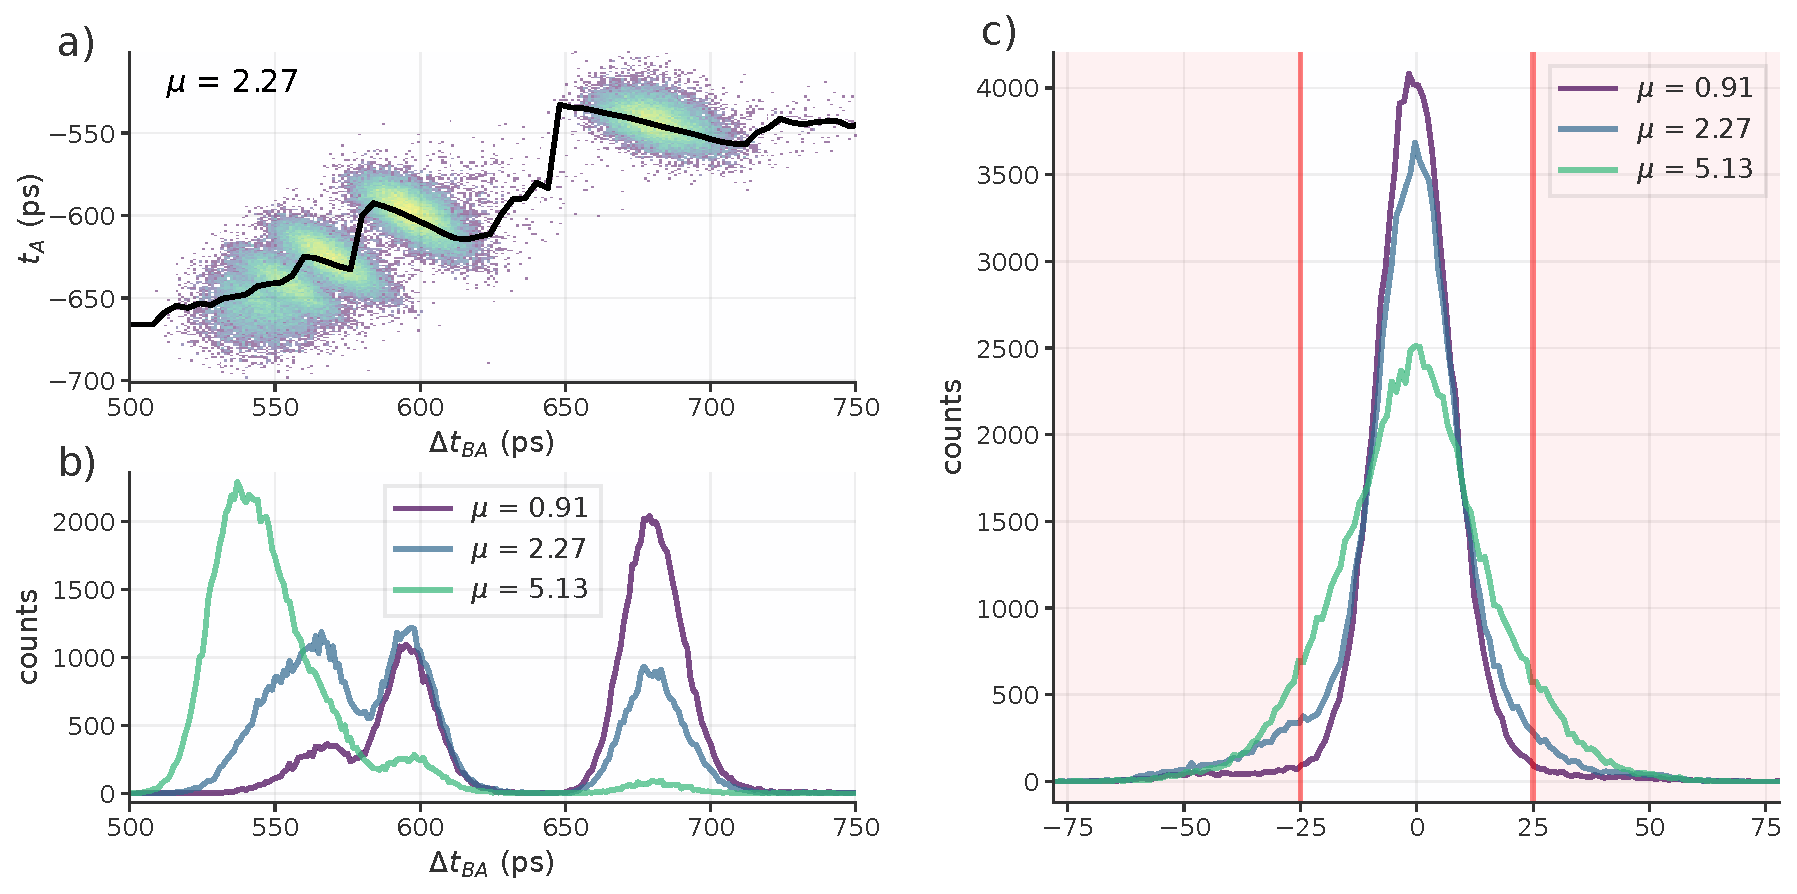
\includegraphics[width=0.75\textwidth,height=\textheight]{chapter_03/figs_03/slope_cancellation_light.pdf}
\caption[{PNR Slope Variation Analysis and Cancellation}]{\textbf{PNR
Slope Variation Analysis and Cancellation} a) 2D histogram of RF pulse
measurements. Through graphing slope \(\Delta t_{BA}\) on the x-axis and
arrival time \(t_A\) on the y-axis, a series of groupings are visible
that identify the discrete photon numbers detected.}
\label{fig:slope-correction}
\end{figure}
}

\hypertarget{cluster-analysis}{%
\subsection{Cluster Analysis}\label{cluster-analysis}}

\hypertarget{results-1}{%
\section{Results}\label{results-1}}

results here

\hypertarget{synchronization-with-a-software-phase-locked-loop-pll}{%
\section{Synchronization with a Software Phase Locked Loop
(PLL)}\label{synchronization-with-a-software-phase-locked-loop-pll}}

\textbf{Todo} \emph{This will be the first place in the thesis that I
introduce the use of my software based phase locked loop (PLL). The
software PLL has been useful in several later projects. I will either
fully explain the PLL here, or I will only introduce and motivate it
here. And a full description will go in an appendix. } 1. For sending
many PPM symbols, I needed a synchronization clock that was (A) always
running, and (B) extremely low jitter. 2. Sending an output from the AWG
to the Swabian timetagger in another room resulted in a less-than-ideal
clock source. The signal was low amplitude, and triggering on it's
rising edge did not make for a very low jitter clock signal. 3. I had
some sense that that should be a way of `averaging' past clock cycles in
some way to cancel jitter. After some research and failed tests toward
developing my own averaging method, I learned a software based Phase
Locked Loop is just what I needed. 4. Initial version was adapted from a
Matlab code on the Phase Locked Loop wikipedia page. That code was
written for a sampled sign wave, but I adapted to take in just one data
point per period. For our non-coherent and time-resolved types of
measurements with SNSPDs, we typically only have clocks of this type.
Where the clock is expressed by some type of optical or RF pulse that
arrives on a regular period. 5. More recently Rahaf Youssef and I have
worked on updating our software PLL tools so that its easier to
understand and reason about, and easier to lock to a given signal.

\hypertarget{outlook-towards-high-rate-pnr-and-time-walk-correction}{%
\section{Outlook: Towards High Rate PNR and Time Walk
Correction}\label{outlook-towards-high-rate-pnr-and-time-walk-correction}}

\hypertarget{high-rate-entanglement-generation}{%
\chapter{High Rate Entanglement
Generation}\label{high-rate-entanglement-generation}}

A version of this chapter is currently under review. A preprint is
released as Chure, G, Kaczmarek, Z. A., and Phillips, R. Physiological
adaptability and parametric versatility in a simple genetic circuit.
bioRxiv 2019. DOI: 10.1101/2019.12.19.878462. G.C. and R.P. designed
experiments and developed theoretical models. G.C. and Z.A.K. collected
and analyzed data. G.C. and R.P. wrote the paper.

\hypertarget{abstract-3}{%
\section{Abstract}\label{abstract-3}}

Entanglement distribution based on time-bins is an attractive option for
emerging quantum networks. We demonstrate a 4 GHz repetition rate source
of photon pairs entangled across early and late time bins separated by
80 ps. Simultaneous high rates and high fidelities are achieved through
multiplexing the Spontaneous Parametric Down Conversion (SPDC) output
into 8 energy-time entangled channel pairs. We demonstrate entanglement
fidelities as high as 99.76\%, total entanglement rates up to 0.5
Mbits/s, and predict a straightforward path towards achieving up to
{\color{darkred} XXX} Mbit/s. Finally, we resolve the density matrices
of individual channels and express distillable entanglement rates in
ebit/s, thereby quantifying the tradeoff between fidelity and
coincidence rates that contributes to useful entanglement distribution.
This source is a fundamental building block for high rate
entanglement-based quantum key distribution systems or advanced quantum
networks.

\hypertarget{introduction-4}{%
\section{Introduction}\label{introduction-4}}

~~~~~

Entangled photons play a vital role in the development of quantum
information processing and communication systems. The ability to
generate entangled photon pairs at a high rate is essential for
establishing reliable and scalable quantum networks, as well as for
implementing entanglement-based quantum key distribution (QKD) systems.
Unlike QKD systems that rely on attenuated lasers, entanglement
distribution systems may fulfill the objectives of QKD while also
serving as the foundation for advanced quantum networks that heavily
rely on entanglement as a fundamental resource.

Entanglement-distribution and entanglement-based QKD systems have been
demonstrated with impressive performance across a number of metrics.
These include 40 Kbps data rates in a QKD system deployed over 50 km of
fiber \autocite{Pelet2022}, as well as multiple polarization entangled
sources that leverage spectral multiplexing. These polarization sources
include a demonstration of 181 kebits/s across 150 ITU channel pairs,
and a high-power source potentially capable of gigabit rates with many
added channels and detectors
\autocite{Alshowkan2022,Neumann2022Entanglement}. Multiple works have
highlighted the need to leverage high total brightness, spectral
brightness, collection efficiency, and high visibility from pair
generating non-linear crystals in order to realize practical high-rate
entanglement distribution \autocite{Neumann2022Entanglement}.

Also, with suitable equipment, robust time-bin modulation is possible
over free space links with turbulence \autocite{Jin2019}. Therefore, the
possibility of simplified fiber-free space interconnects and larger
quantum networks based on a shared time-bin protocol motivates
development of improved time-bin sources.

We employ a 4.0 GHz mode locked laser source with 80-ps delay
interferometers to realize a high-rate source. Wavelength multiplexing
is used for reading out energy-time entangled photon pairs, thereby
realizing multiple high fidelity channels pairings which together sum to
a high coincidence rate. Each of the 8 pairs can be considered an
independent carrier of photonic entanglement \autocite{Wengerowsky2018}
and therefore the system as a whole is applicable to flex-grid
architectures through the use of wavelength selective switching
\autocite{Appas2021,Alshowkan22Switching}. However, we focus here on
maximizing the rate between two receiving stations, Alice and Bob
(Fig.~\ref{fig:system} a). Each station is equipped with DWDMs that
receive multiplexed channels, and may include multiple detectors to read
out the full rate.

\hypertarget{fig:system}{%
\begin{figure}
\centering
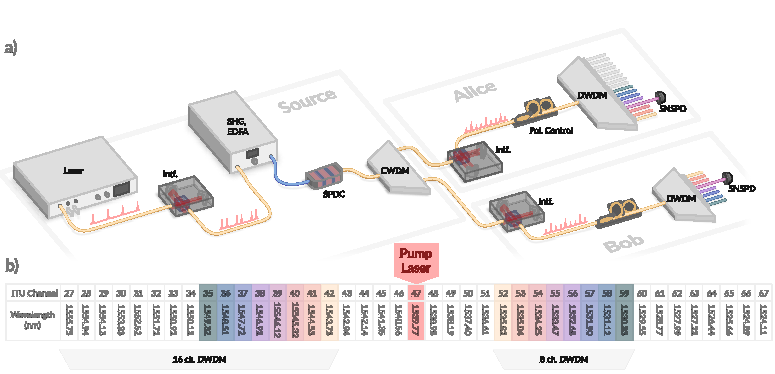
\includegraphics[width=1\textwidth,height=\textheight]{chapter_04/figs_04/sys_drawing_light.pdf}
\caption[{System Drawing \& DWDM Channels.}]{\textbf{System Drawing \&
DWDM Channels} a) Pulses from a 1539.47 nm mode locked laser (Pritel
UOC) are doubled by an 80 ps delay interferometer before up-conversion
and amplification in a SHG \& EDFA module (Pritel). A short PM fiber
from the SHG connects to the SPDC where photon pairs are created. The
CWDM module separates the SPDC spectrum into multiple
\(\sim\!\!13~\mathrm{nm}\) wide bands spaced by 20 nm. The 1530 and 1550
nm bands are sent to the Bob and Alice stations respectively. The
readout interferometers have the same time delay as the source
interferometer. Polarization controllers are used to maximize the
coincidence rates, as the detection efficiencies of the SNSPDs is
polarization sensitive \(\pm20\%\). Entanglement fidelity is unaffected
by readout polarization. The two SNSPDs are connected to each channel
pair in succession to resolve full system performance. b) ITU channels
involved with the experiment. Pairs of channels highlighted with the
same color obey the SPDC \& pump energy matching condition, and can be
directly read out through DWDM channel outputs. To asses the full 16
channels (27-42) of Alice's DWDM multiplexer, Bob's 8-channel DWDM is
switched out for a tunable narroband filter.}
\label{fig:system}
\end{figure}
}

We quantify per-channel brightness and fidelity as a function of pump
power, as well as collection efficiencies, coincidence rates across 8
channel pairs, and expected performance of a partially realized
16-channel pair configuration. We show that the 8 channel system
achieves low-power fidelities that average to 99.76\%. At a higher
power, we demonstrate a total coincidence rate of 0.51 MHz with
fidelities that average to 99.22\%. Through quantum state tomography we
bound the distillable entanglement rate of the system to between 80\%
and 95\% of the high-power coincidence rate (0.41 - 0.48 Mebits/s).

Quantifying a source's spectral mode purity is important for gauging its
utility in advanced quantum networks that rely on 2-photon interference
measurements like Bell State Measurements.

With Schmidt decomposition we quantify the modal purity of single DWDM
channel pairs and derive the inverse Shmidt number which serves as an
estimate for two-photon HOM visibility between two such sources.
Ultimately, we demonstrate that an entanglement generation source of
this design makes for a robust and powerful building block for future
high rate quantum networks.

\hypertarget{system}{%
\section{System}\label{system}}

Figure \href{./section_03_introduction.md\#fig:system}{system} shows the
experiment setup. Pulses from a 4 GHz mode locked laser (Pritel UOC)
with a center wavelength at 1539.47 nm are sent through an 80 ps delay
interferometer (Optoplex). This generates the early/late basis, which is
subsequently unconverted by a second harmonic generation (SHG) module
(Pritel) and down converted into entangled photon pairs by a type-0
spontaneous parametric down conversion crystal (Covesion). The
up-converted pulses at 769 nm have a FWHM bandwidth of 243 GHz (0.48
nm), which along with the phase matching condition of the SPDC
waveguide, defines a wide Joint Spectral Intensity (JSI) function.

The entangled pairs, which are separated by a coarse wavelength division
multiplexer (CWDM), are of the form
\(|\psi\rangle=\frac{1}{\sqrt{2}}\left(|1\rangle_{s}|1\rangle_{i}+e^{i \phi}|2\rangle_{s}|2\rangle_{i}\right)\).
Entangled idler and signal photons are sent to the receiving stations
labeled Alice and Bob. One readout interferometer at each station
projects all spectral bands into a composite time-phase basis. From
here, dense wavelength division multiplexers (DWDM) divide up the
energy-time entangled photon pairs into spectral channels.

The outputs of the DWDMS are sent to differential niobium nitride (NbN)
superconducting nanowire single photon detectors (SNSPDs)
\autocite{Colangelo2023} with efficiencies of \textcolor{red}{XX} and
\textcolor{red}{XX}. These measure the arrival time of photons with
respect to a clock signal derived from the mode locked laser. We use two
SNSPDs for this demonstration, but a full 8-channel implementation of
this system requires 16 detectors operating in parallel at both Alice
and Bob. To read out both outputs of both interferometers, 4 detectors
per channel are required.

\hypertarget{results-2}{%
\section{Results}\label{results-2}}

The JSI is measured in Fig. Fig.~\ref{fig:jsi} a by recording
coincidence rates for different ITU channel pairings. For a given idler
photon wavelength, the spectrum of corresponding signal photons spans
several ITU channels. Pairs along the main diagonal are optimized for
maximum coincidence rates, and are therefore used for all remaining
measurements. In \href{./section_03_introduction.md\#fig:system}{system}
c, these pairs are highlighted with matching colors.

\hypertarget{fig:jsi}{%
\begin{figure}
\centering
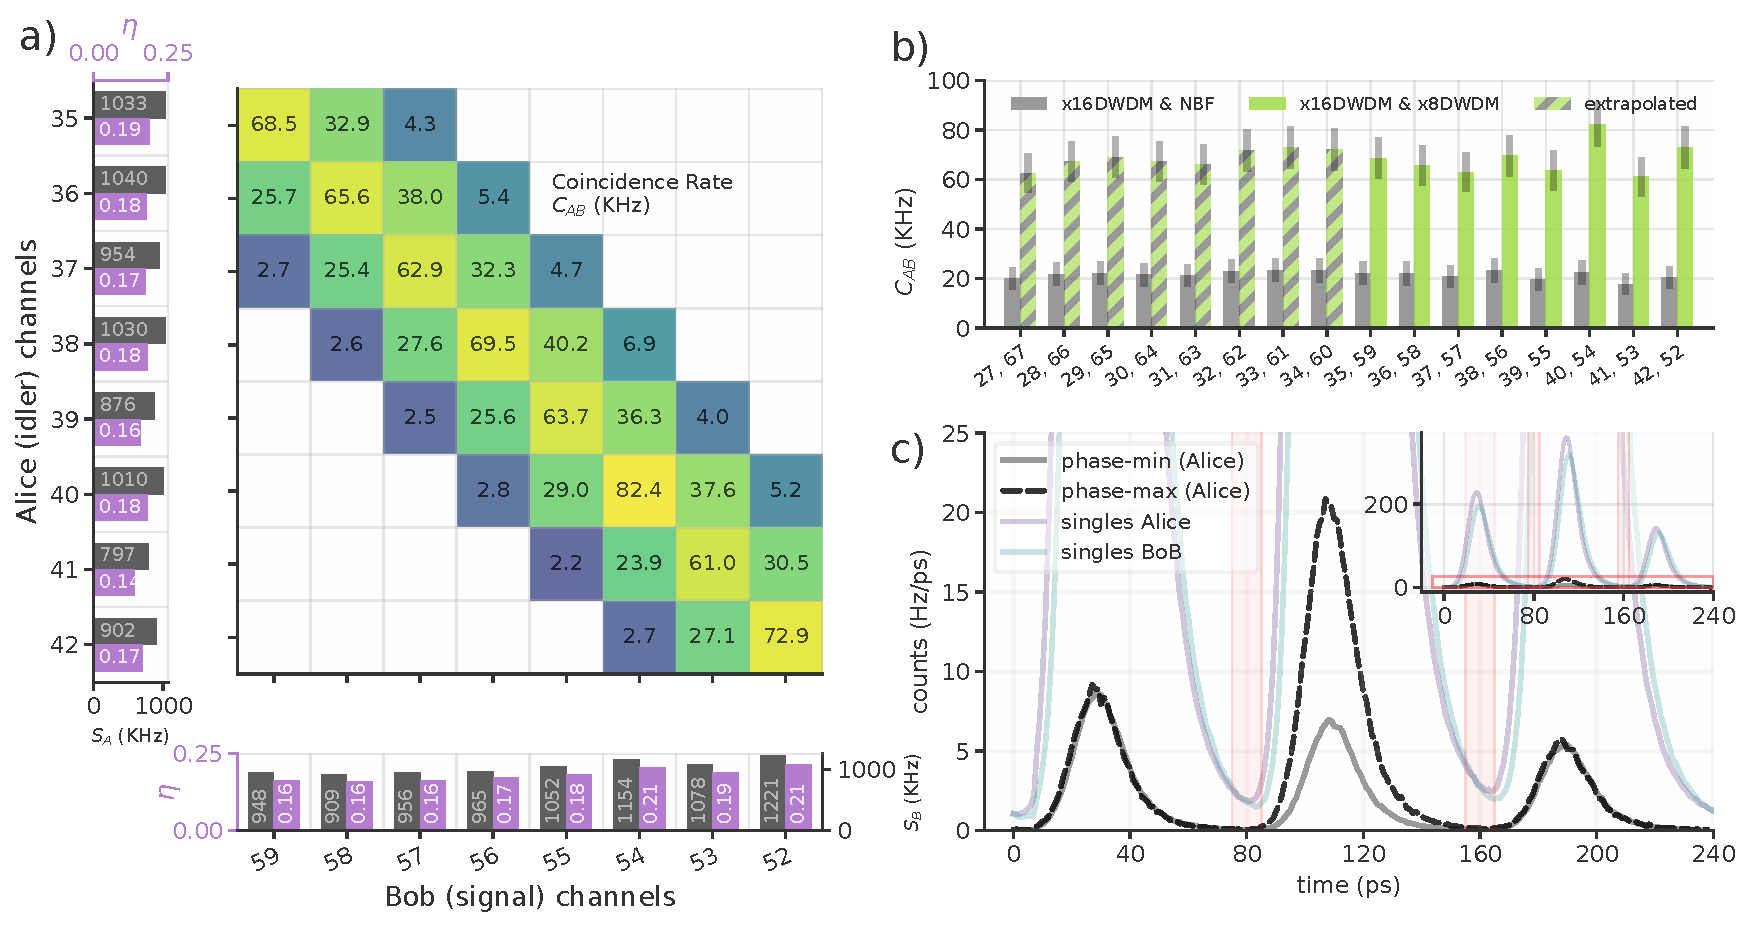
\includegraphics[width=1\textwidth,height=\textheight]{chapter_04/figs_04/jsi_figure_light.pdf}
\caption[{Channel JSI and Histogram.}]{\textbf{Channel JSI and
Histogram} a) The singles rates \(S_A\) and \(S_B\) (grey bars),
coupling efficiencies (purple bars), and coincidence rates \(C_{AB}\)
(diagonal boxes) for different DWDM channel pairings. The joint spectral
intensity envelop spans several 100 GHz channels. So the coincidence
rates (KHz, in black) are consistent with the efficiencies \(\eta\)
(purple bars) and the singles rates (grey bars), they are scaled to
represent two branches of the total wavefunction. There are four
branches in all, for the 4 pairs of 2 interferometer output ports that
contribute coincidences. In practice, one output each of Alice and Bob's
interferometers is measured, thereby capturing one branch. See
supplemental for details of the scaling method, and the fitting method
used to solve for the coupling efficiencies \(\eta\). b) Coincidence
rates for energy-matched channel pairings. The light green bars match
the main diagonal in (a). Grey bars are measured with x16 DWDM at Alice
and a tunable narroband filter at Bob. Dashed bars predict the rates for
a system with x16 DWDMs at both Alice and Bob c) Histogram of photon
arrival events with respect to the 4 GHz clock. Dashed black and grey
lines show the response functions for coincidence events. Red bars
represent guard regions where coincidence events are ignored.}
\label{fig:jsi}
\end{figure}
}

Figure Fig.~\ref{fig:jsi} a also shows coupling efficiencies \(\eta\)
for each DWDM channel, \(S_A\) is the singles rate at Alice, and \(S_B\)
is the singles rate at Bob \autocite{Neumann2022Entanglement}. As only
two of the total four interferometer output ports are measured at once,
certain scalings are made to the singles and coincidence rates
\(C_{AB}\) to reflect a readout configuration with well defined coupling
efficiency (see supplementary information).

Most tests were done with the 8 ITU 100 GHz channel pairings: Ch. 35-42
at Alice and Ch. 52-49 at Bob. In Fig. Fig.~\ref{fig:jsi} b we
investigate rates across 16 pairs by using all 16 channels available on
the DWDM at Alice (24 - 34) and a tuneable narroband filter in place of
the DWDM at Bob. As the narroband filter has higher loss, the
coincidence rates are lower (grey bars in Fig. Fig.~\ref{fig:jsi} b).
But the uniformity of coincidence rates across 16 channels implies the
use of 16-channel DWDMs at both Alice and Bob would roughly double the
total coincidence rate.

Signals from the SNSPDs are read out with a free running time tagger
(Swabian) and processed with custom software. In the resulting
histograms referenced from a shared clock (Fig Fig.~\ref{fig:jsi} c),
three peaks are visible which are caused by the sequential delays of the
source and readout interferometers. Some intensity imbalance between
long and short paths is present in these interferometers, which explains
the asymmetry between early and late peaks in Fig.~\ref{fig:jsi} c.~This
type of imbalance is expected to degrade entanglement fidelity only if
present in the source interferometer (see supplemenatry info).
Therefore, that with lowest imbalance was chosen for the source.

The coincidence rate across Alice and Bob's middle bins varies
sinusoidally with respect to the combined phase relationship source and
readout interferometers (see supplementary information)
\autocite{Inagaki2013}. In figure Fig.~\ref{fig:jsi} c the coincidences
shown are for any combination of early, middle, or late bins. For
tomography and fidelity measurements, coincidences across specific bin
pairings are considered. Events within 10 ps width guard regions
centered at 80 and 160 ps (shaded red) are discarded for analysis of
coincidences between individual bins. This is done to maximize fidelity
in the presence of some minor overlap of the pulse response functions.

\hypertarget{fig:shg_scan}{%
\begin{figure}
\centering
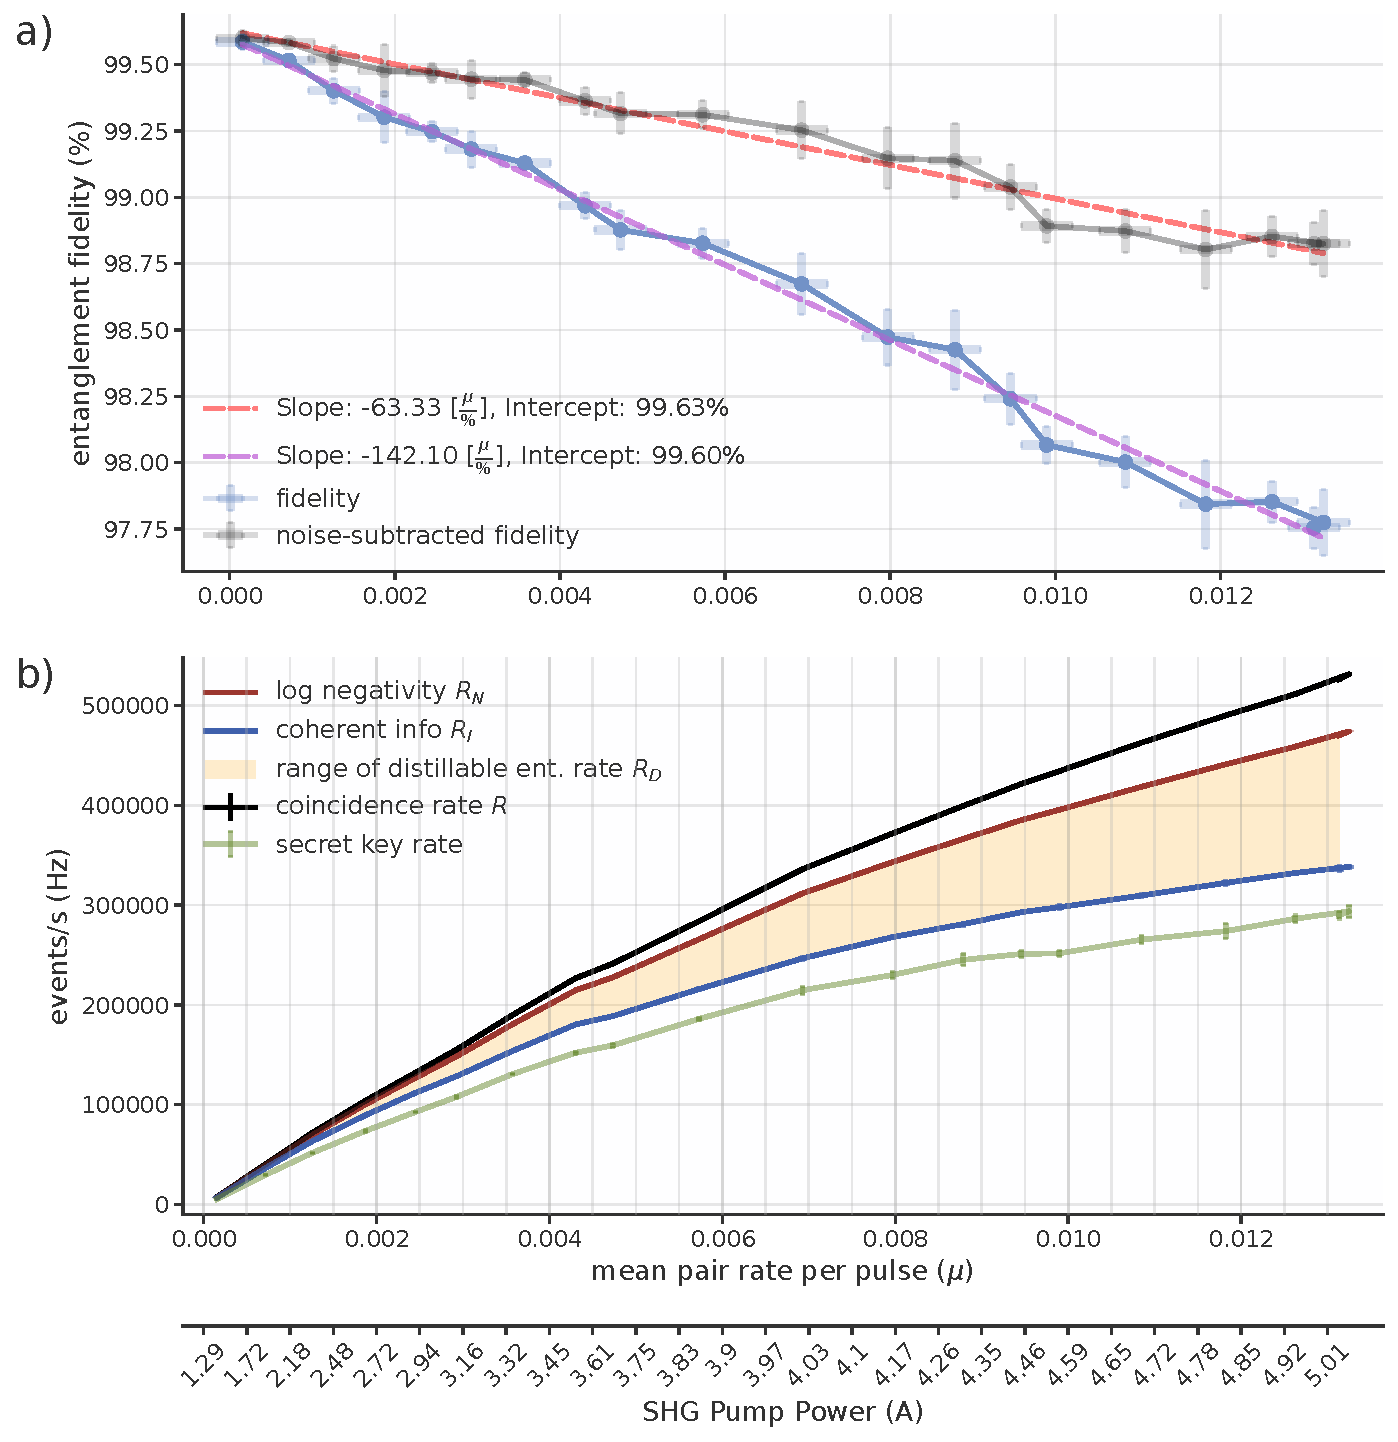
\includegraphics[width=1\textwidth,height=\textheight]{chapter_04/figs_04/shg_scan_light.pdf}
\caption[{Fidelity and Rates vs \(\boldsymbol \mu\).}]{\textbf{Fidelity
and Rates vs \(\boldsymbol \mu\)} a) Fidelity versus pump power. Error
bars arise from making multiple measurements of the center bin
coincidence rate over some integration time. These measurements span
small ranges of interferometer phase, as the extremum-finding algorithm
jitters the interferometer voltage. b) Bounded distillable entanglement
rate versus pump power. Multiple such measurements are made for all the
tomographic measurements. These are used to calculate standard
deviations for fidelity, log negativity, and coherent information. Error
bars for the log negativity and coherent information are smaller than
the line width shown. Rates shown assume readout of all 4 available
interferometer ports, based on data measured using one port each at
Alice and Bob.}
\label{fig:shg_scan}
\end{figure}
}

Due to the small size and athermal design of the interferomters, minimal
temporal phase drift was observed over multiple hours. Nevertheless,
software was used to `lock' the phase at a minimum or maximum with a
simple steepest-descent algorithm. This varied the phase by small
amounts over several minutes and adjusted phase to maintain an extremum.

Channels 35 and 59 were chosen for an analysis of entanglement fidelity
and rates versus pump power. Fidelity with respect to pump power or mean
entangled pair rate is shown in Fig.~\ref{fig:shg_scan} a. We define the
entanglement fidelity as \(F = 100\%*(1 - \frac{C_{min}}{C_{max}})\)
where \(C_{min}\) and \(C_{max}\) are the minimum and maximum
coincidence rates with respect to interferometer phase observed across
the middle bins. As this coincidence rate depends on the total phase
across all source and readout interferometers, just one (Bob's) is
actively controlled to scan the full state space.

\hypertarget{fig:channel_data}{%
\begin{figure}
\centering
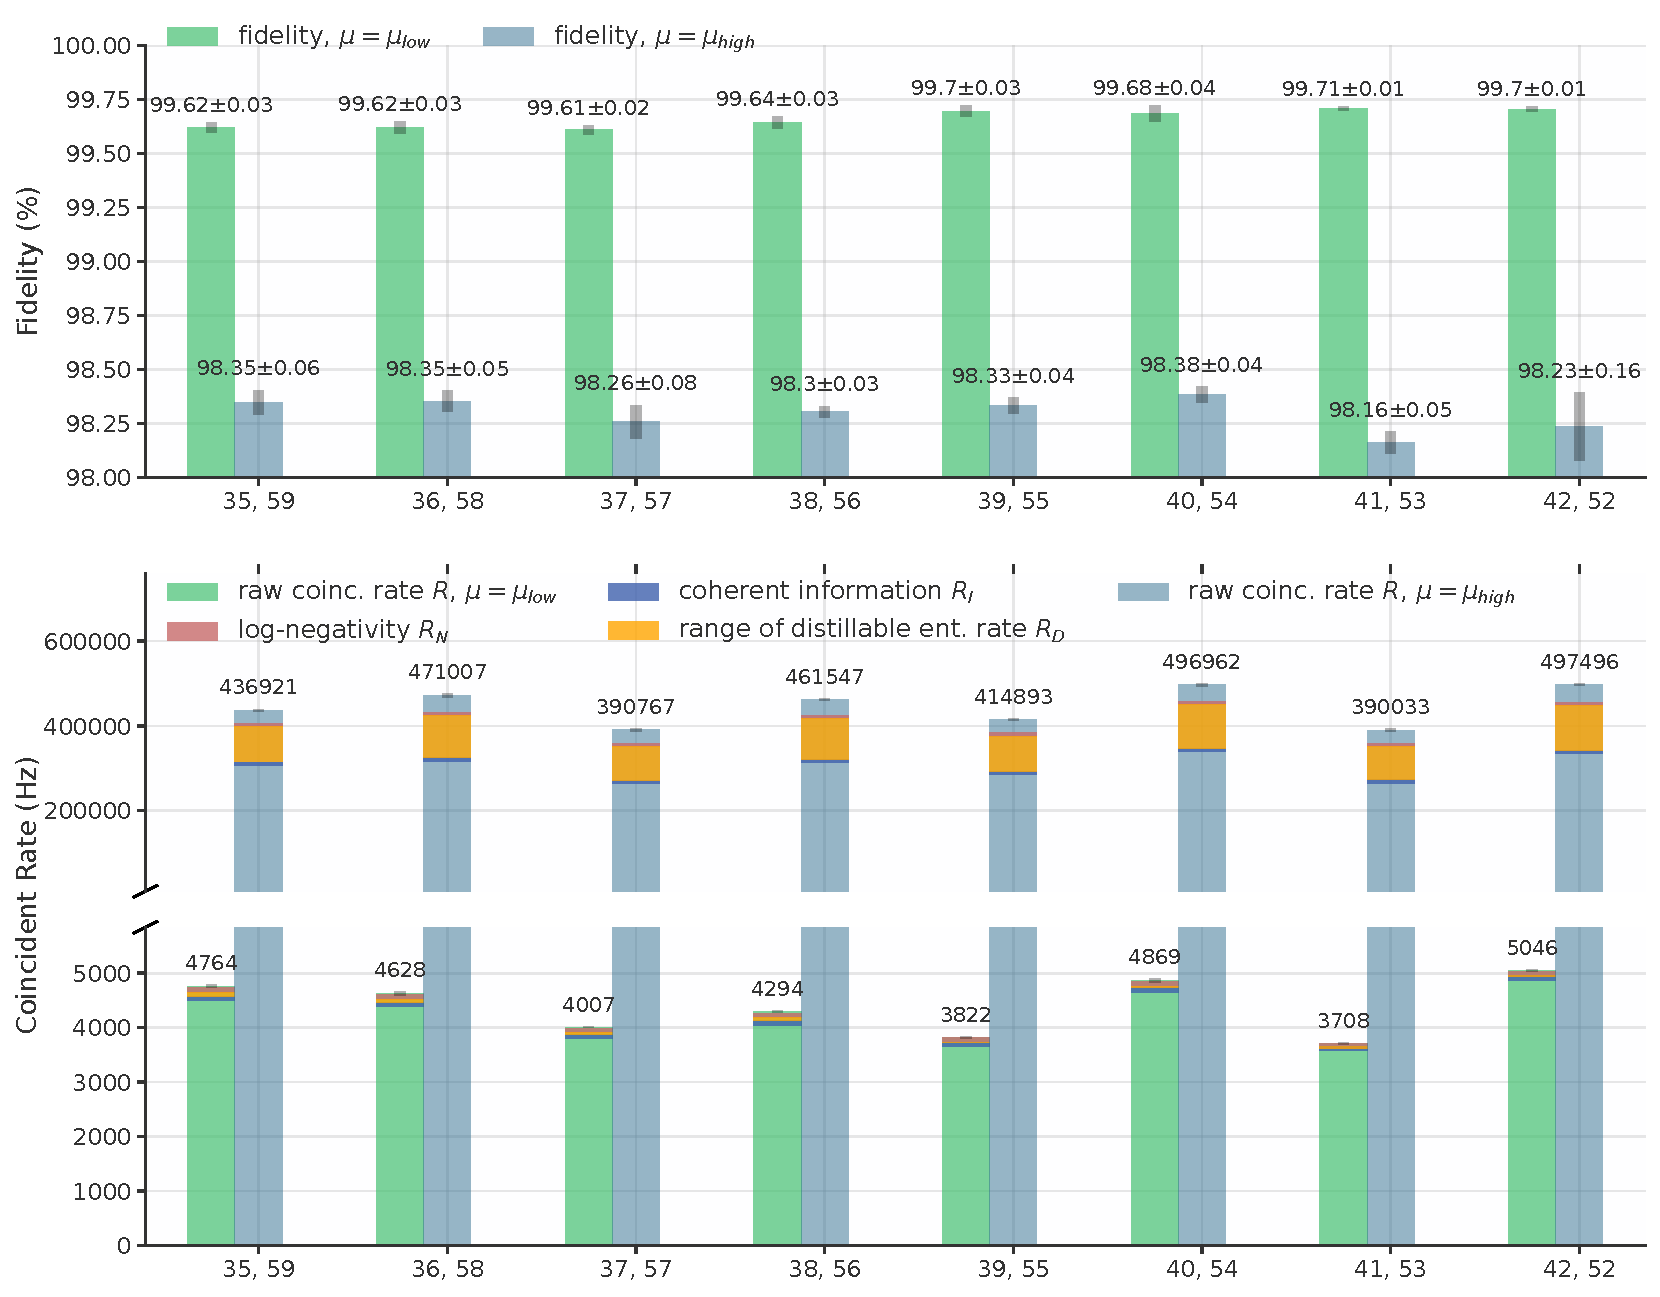
\includegraphics[width=1\textwidth,height=\textheight]{chapter_04/figs_04/8ch_bar_graph_high_power_light.pdf}
\caption[{Fidelity and rates across 8 channel pairs.}]{\textbf{Fidelity
and rates across 8 channel pairs} a) Fidelity for the main 8 channel
pairs, measured at a high (5.17 Amps) and a low ( 1.2 Amps) SHG pump
power setting. Each power setting results in similar \(\mu\) for all
channels: \(\mu_{low}\) = 5.6e-5 \(\pm\) 9e-6 and \(\mu_{high}\) =
6.1e-3 \(\pm\) 3e-4. b) Rate metrics for the 8 channel pairs at the same
high and low power settings. The range of possible values for
distillable entanglement rate is spanned by the yellow regions, bounded
above by log-negativity and below by coherent information. Rates shown
assume readout of all 4 available interferometer ports, based on data
measured using one port each at Alice and Bob}
\label{fig:channel_data}
\end{figure}
}

We quantify the rate of useful entanglement by supplying bounds for the
distillable entanglement rate \(R_D\). Measured in ebits/s, \(R_D\) is
the maximal asymptotic rate of Bell pair production per received state
using only local operations and classical communications. It is bounded
above by log negativity \(R_N = RE_N\) and below by \(R_I = R E_I\)
where \(R\) is the raw coincidence rate \autocite{Alshowkan2022}. For
each pump power setting in Fig.~\ref{fig:shg_scan}, a series of
tomographic measurements is performed and density matrices calculated.
\(E_I\) and \(E_N\) are calculated from the density matrices as detailed
in the supplementary information.

Figure Fig.~\ref{fig:channel_data} shows fidelities, raw coincidence
rates, and bounded distillable entanglement rates for all 8 channel
pairings and 2 pump powers. The higher pump power is the highest
possible on our SHG \& EDFA module. Higher rates are readily achievable
by increasing the output power of this component, up to a point where
the high count rate on the SNSPDs induces higher jitter. However these
pulse pileup and time-walk effects can be mitigated with jitter
correction techniques \autocite{Mueller2023}.

\% \textbackslash textcolor\{blue\}\{ \% We perform a linear fit of the
entanglement fidelity data, \(F = A + B\mu\), and obtain \(A = XXX\),
\(B=XXX\). We derive expressions for A and B in terms of the mean photon
number, interferometer transmittances, and interference visibilities
(see Supplemental).\}

Using the data in Fig. Fig.~\ref{fig:jsi} a, we model the joint spectral
intensity function of the SPDC output as a product of pump envelope and
phase matching condition functions

\[|f(\omega_s, \omega_i)|^2 = |\psi_{\mathrm{ph}}\left(\omega_s, \omega_i\right)|^2 *|\psi_p\left(\omega_s, \omega_i\right)|^2\]

This construction depends on the wavelength (769.78 nm) and bandwidth
(243 GHz FWHM) of unconverted light out of the SHG, which was measured
with a spectrum analyzer. The transmission spectrums of the 100 GHz DWDM
channels was also modeled based on measured transmission data, in order
to define the integrations over the JSI that would match the coincidence
results in Fig. Fig.~\ref{fig:jsi} a (details in supplemental).

We calculate the Schmidt decomposition of the JSI bipartite spectrum
transmitted through pairs of DWDM filters at Alice and Bob, and derive
an inverse Schmidt number of \(1/K = 0.87\). This value quantifies the
spectral purity of the entangled photon source, and predicts the
visibility of a two-source HOM (Hong-Ou-Mandel) interferogram. If 50 GHz
ITU channels are used instead, the model predicts \(1/K = 0.96\).

\appendix

In March of 2022, Matthew Shaw was a guest lecturer for the Quantum
Hardware and Techniques course (APh/Ph 138b). The following is a
homework assignment I wrote to accompany his series of lectures.

The first problem is inspired by the low dark count rate
publication\autocite{Mueller:21}. It has the student build a simple
model for a dark count rate transmitted through a series of filters.
Finally, it leads the student to consider an ultimate tradeoff between
dark count rate and coupling efficiency to wide bandwidth optical
signals. A filtering system that only transmits a very narroband signal
will not be able to detect ultra-short optical signals with high
efficiency or temporal resolution.

The second problem explores a potential use case of a photon number
resolving SNSPD. It closely follows logic presented in an Andreas Christ
and Christine Silberhorn paper\autocite{Andreas:12}. I studied this
paper earlier in my PhD, when I considered developing a multiplexed
single photon source. It turned out that project was overly ambitious,
but future PhD students might consider approaching it again.

\textcolor{midnightblue}{Contact
\href{mailto:andrewstermueller@gmail.com}{Andrew Mueller} with any
questions about the homework or solution manual. The solutions to some
sections specify finer-grained point values when there are multiple
answers per section. As the grader, feel free to use these or not. }

\hypertarget{free-space-coupling-with-low-dark-counts-50-points}{%
\subsection{1. Free space coupling with low dark counts (50
points)}\label{free-space-coupling-with-low-dark-counts-50-points}}

An experimental apparatus emits a collimated beam of
\(1550~\mathrm{nm}\) photons with gaussian beam waist
\(w_0 = 3~\mathrm{mm}\). You wish to focus the beam onto an SNSPD
directly through a window in a cryostat.

\hypertarget{fig:cryostat_concept}{%
\begin{figure}
\centering
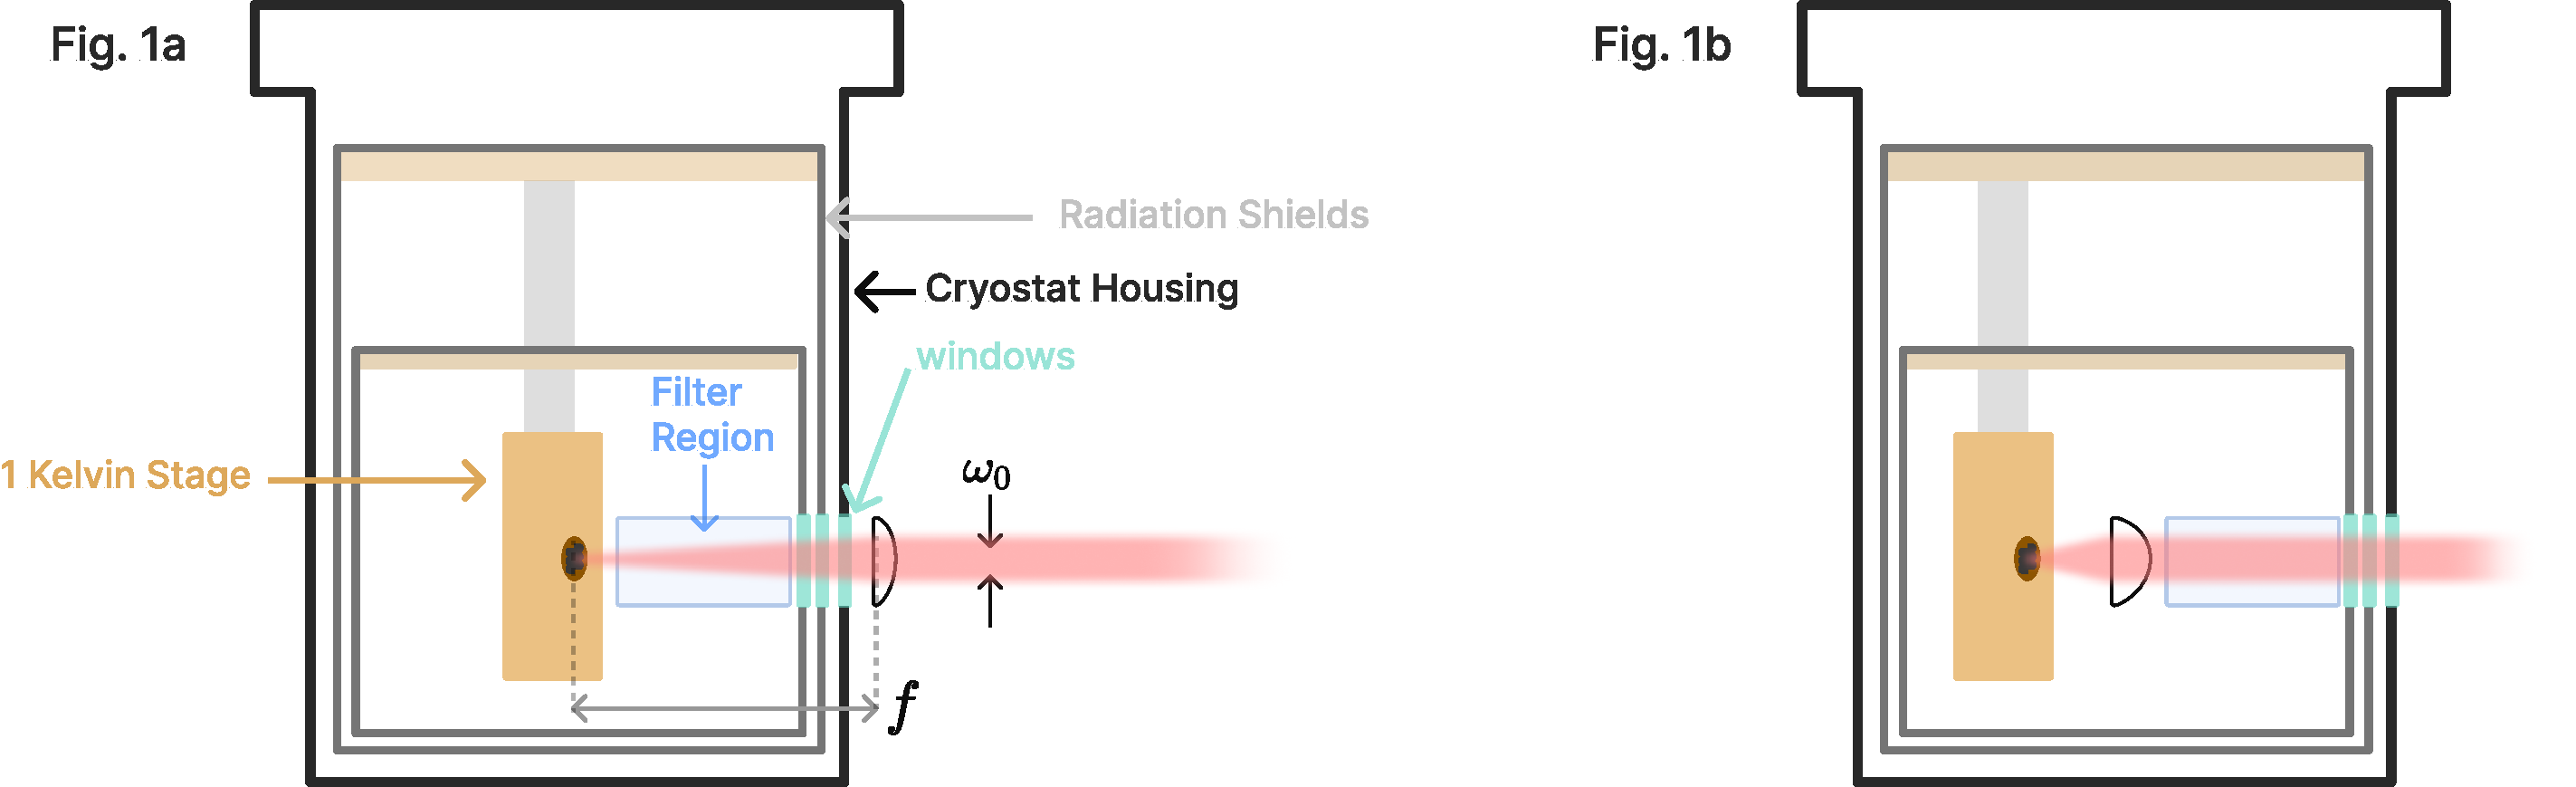
\includegraphics{chapter_05/figs_05/fig1b_light.pdf}
\caption[{Cryostat optical coupling}]{\textbf{Cryostat free space
coupling options.}}
\label{fig:cryostat_concept}
\end{figure}
}

As we will see later on, a set of filters will be needed between the
detector and the window to minimize dark counts. In practice, the set of
filters can be quite thick. Say a \(f = 100~\mathrm{mm}\) lens is used
right outside the cryostat to focus the beam onto the detector though a
set of filters (Fig.~\ref{fig:cryostat_concept} a). The long focal
length makes room for a few inches of filters between the external lens
and focused spot.

\begin{enumerate}
\def\labelenumi{\arabic{enumi}.}
\item
  (4 pts) If the detector has a circular active area with radius
  \(5~\mathrm{\upmu m}\), what ratio of power in the beam can it
  collect? Assume the detector has unity efficiency across all angles of
  incidence with respect to the surface normal.

  \textcolor{midnightblue}{

  \textbf{Answer:}

  }

  \textcolor{midnightblue}{

  The divergence angle of the guassian beam:
  \(\theta = \tan^{-1}({\frac{3}{100}})\).

  }

  \textcolor{midnightblue}{ The formula for divergence angle in terms of
  waist \(w_0\): \(\theta = \frac{\lambda}{\pi w_0}\) }

  \textcolor{midnightblue}{ Combining and plugging in, the waist radius
  at focus is
  \(\frac{1550~\mathrm{nm}}{\pi \tan^{-1}(\frac{3}{100})} \approx 16.5~ \mathrm{\upmu m}\)
  }

  \textcolor{midnightblue}{ The formula for power inside an aperture at
  \(w(z)\) for a guassian beam:}

  \textcolor{midnightblue}{

  \[P(r, z)=P_{0}\left[1-e^{-2 r^{2} / w^{2}(z)}\right]\]

  }

  \textcolor{midnightblue}{We are interested in the ratio of power
  collected at \(w(z=0) = w_0\) which may be expressed as:}

  \textcolor{midnightblue}{

  \[P(r, z=0)=1-e^{-2 r^{2} / w_0^{2}}\]

  }

  \textcolor{midnightblue}{Plugging in: }

  \textcolor{midnightblue}{

  \[P(r, z=0)=1-e^{-2(5^{2}) / 16.5^{2}} \approx  \boxed{0.17} \]

  }
\item
  (4 pts) A faster lens mounted much closer to the detector inside the
  cryostat focuses to a smaller waist. Consider an
  \(f = 18~\mathrm{mm}\) lens with the detector at the focal length
  (Fig.~\ref{fig:cryostat_concept} b). Verify more than 99\% of the
  collimated light will be focused onto the active area of the detector.

  \textcolor{midnightblue}{ The waist radius at focus is
  \(\frac{1550~\mathrm{nm}}{\pi \tan^{-1}(\frac{3}{18})} \approx 2.98~\mathrm{\upmu m}\)
  }

  \textcolor{midnightblue}{Ratio of power within the
  \(10~\mathrm{\upmu m}\) radius active area: }

  \textcolor{midnightblue}{

  \[P(r, z=0)=1-e^{-2(5^{2}) / 2.98^{2}} \approx \boxed{0.996} \]

  }

  Without filtering, the mid-infrared photons coupled to the detector
  from the room temperature laboratory are a dominant source of dark
  counts. Think of the environment outside the window as an isotropic
  blackbody emitter. Consider 3 cases, where the shaded red regions
  illustrate the light field of thermal radiation that could couple to
  the detector:

  \hypertarget{fig:coupling_options}{%
  \begin{figure}
  \centering
  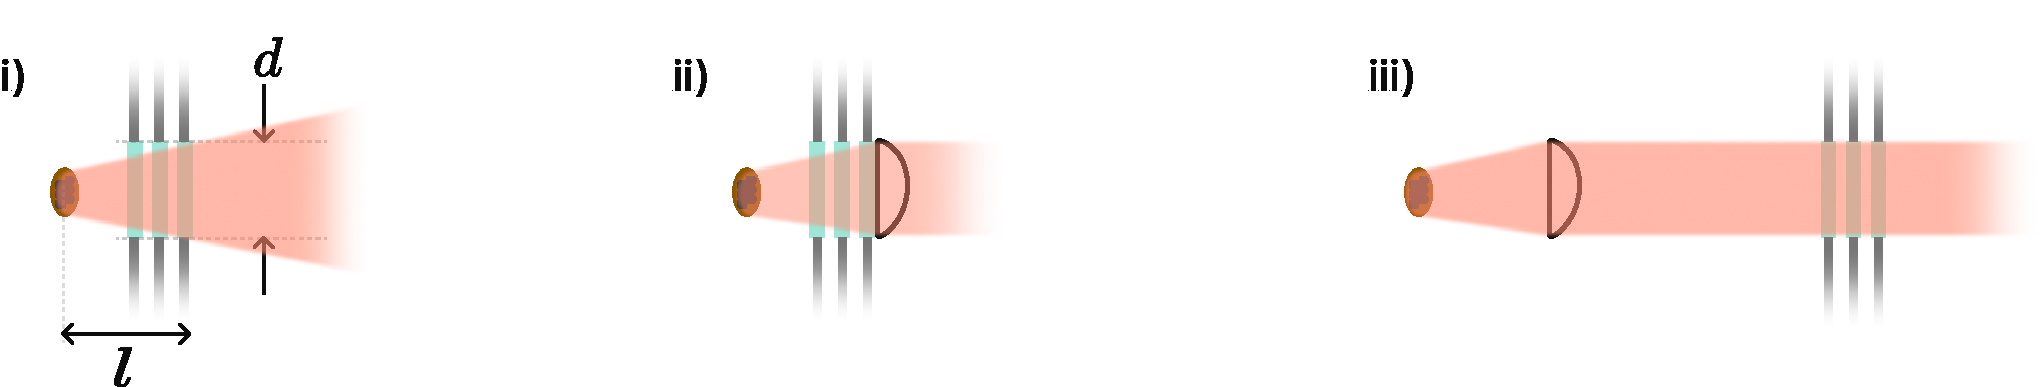
\includegraphics{chapter_05/figs_05/fig2b_light.pdf}
  \caption[{Cryostat coupling options}]{\textbf{Three Coupling Options}}
  \label{fig:coupling_options}
  \end{figure}
  }

  \begin{enumerate}
  \def\labelenumii{\roman{enumii})}
  \tightlist
  \item
    There is no lens; the detector is distance \(l\) inside the
    cryostat, and the first window with diameter \(d\) defines an
    entrance pupil.
  \item
    Same as (i), but a lens with focal length \(l\) is placed right
    outside the first window. The detector is at the focal point.
  \item
    Same as (ii) but the lens is placed inside the cryostat with the
    detector still at the focal length. Equivalent to
    Fig.~\ref{fig:cryostat_concept} b above.
  \end{enumerate}
\item
  (6 pts) Does (ii) couple more, less, or equal dark counts to the
  detector than (i)? What about case (iii)? Why? No calculations should
  be needed. (Hint: Consider the units of radiance, which characterizes
  a black body emitter. Etendue or beam parameter product may be useful
  concepts to consider)

  \textcolor{midnightblue}{ \textbf{Answer:} } \textcolor{midnightblue}{
  The three cases couple the same amount of light to the detector. (ii)
  couples the same amount of power as (i) because a blackbody source
  can't be focused to higher intensity with a lens. The solid angle
  subtended by the entrance pupil as seen by the detector is the same in
  all cases. The detector area stays the same as well so the etendue is
  conserved across all three cases. This implies the same radiant power
  is coupled. }

  \textcolor{midnightblue}{ 3 points for saying all situations couple
  the same rate; 3 points for some explanation. }
\item
  (9 pts) Using Planck's law with laboratory temperature \(T\) and the
  geometry of case (i) above, write an expression for spectral radiant
  flux (photons per unit wavelength) on the active area of a detector
  with radius \(r\).

  \textcolor{midnightblue}{ \textbf{Answer:} }
  \textcolor{midnightblue}{The expression is a product of several
  factors:}

  \textcolor{midnightblue}{

  \[\text{Flux}[\lambda] = P \Omega D_{area} B_{\lambda}(\lambda, T)\]

  }

  \textcolor{midnightblue}{ Where \(P = \frac{\lambda}{hc}\) is the
  number of photons per unit energy, \(\Omega\) is the solid angle of
  blackbody radiation as seen by the detector, \(D_{area} = \pi r^2\) is
  the area of the detector, and \(B_{\lambda}\) is Planck's law. }
  \textcolor{midnightblue}{Planck's law:}

  \textcolor{midnightblue}{

  \[B_{\lambda}(\lambda, T)=\frac{2 h c^{2}}{\lambda^{5}} \frac{1}{e^{h c /\left(\lambda k_{\mathrm{B}} T\right)}-1}\]

  }

  \textcolor{midnightblue}{ \(\Omega = \pi \sin{\theta^2}\), where
  \(\theta = \tan^{-1}(\frac{(d/2)}{l})\) is the half angle of the field
  of view of blackbody radiation as seen by the detector. }

  \textcolor{midnightblue}{The full expression: }

  \textcolor{midnightblue}{

  \[\text{Flux}[\lambda] = \frac{\lambda \pi^2 r^2 \sin{\theta^2}}{hc} \frac{2 h c^{2}}{\lambda^{5}} \frac{1}{e^{h c /\left(\lambda k_{\mathrm{B}} T\right)}-1}, \,\,\,\,\,\,\,\,\,\,\,\theta = \tan^{-1}(\frac{(d/2)}{l})\]

  }

  \textcolor{midnightblue}{ Since the expression asked for can be
  written many ways, just verify the student has taken into account all
  the terms in equation (1) above, and has the correct expressions for}
  \textcolor{darkred}{\(\Omega\) (3 pts), \(\theta\) (3 pts), and P (3
  pts).}
\item
  (6 pts) Consider the configuration in Fig. 1b). The detector has an
  internal quantum efficiency approximated by:

  \[\eta(\lambda) = \frac{1}{2}(1 - \text{erf}[\lambda - 3~\mathrm{\upmu m}]) \]

  \(\lambda\) is measured in \(\mathrm{\upmu m}\) and \(\text{erf}()\)
  is the error function. Using your conclusions from (1.3) and
  expression from (1.4), write a formula \(N_{photons}[\lambda]\) for
  the number of detectable dark counts with respect to \(\lambda\), then
  numerically integrate it to find the dark count rate with no
  filtering. The laboratory temperature \(T\) is 293 K, lens focal
  length \(l\) is \(18~\text{mm}\), detector radius \(r\) is
  \(5~\mathrm{\upmu m}\), and the diameter \(d\) of all optics is 1
  inch. The maximum count rate of this SNSPD is 10 MHz. Is the detector
  usable or overexposed?

  \textcolor{midnightblue}{ \textbf{Answer:} }
  \textcolor{midnightblue}{Use the expression from (1.4) and multiply it
  by the quantum efficiency function \(\eta(\lambda)\) }

  \textcolor{midnightblue}{

  \[N_{photons}[\lambda] = P \Omega D_{area} \eta(\lambda) B_{\lambda}(\lambda, T=293)\]

  }

  \textcolor{midnightblue}{ Here is the function expressed in mathmatica
  and the solution to the integral: }

  \textcolor{midnightblue}{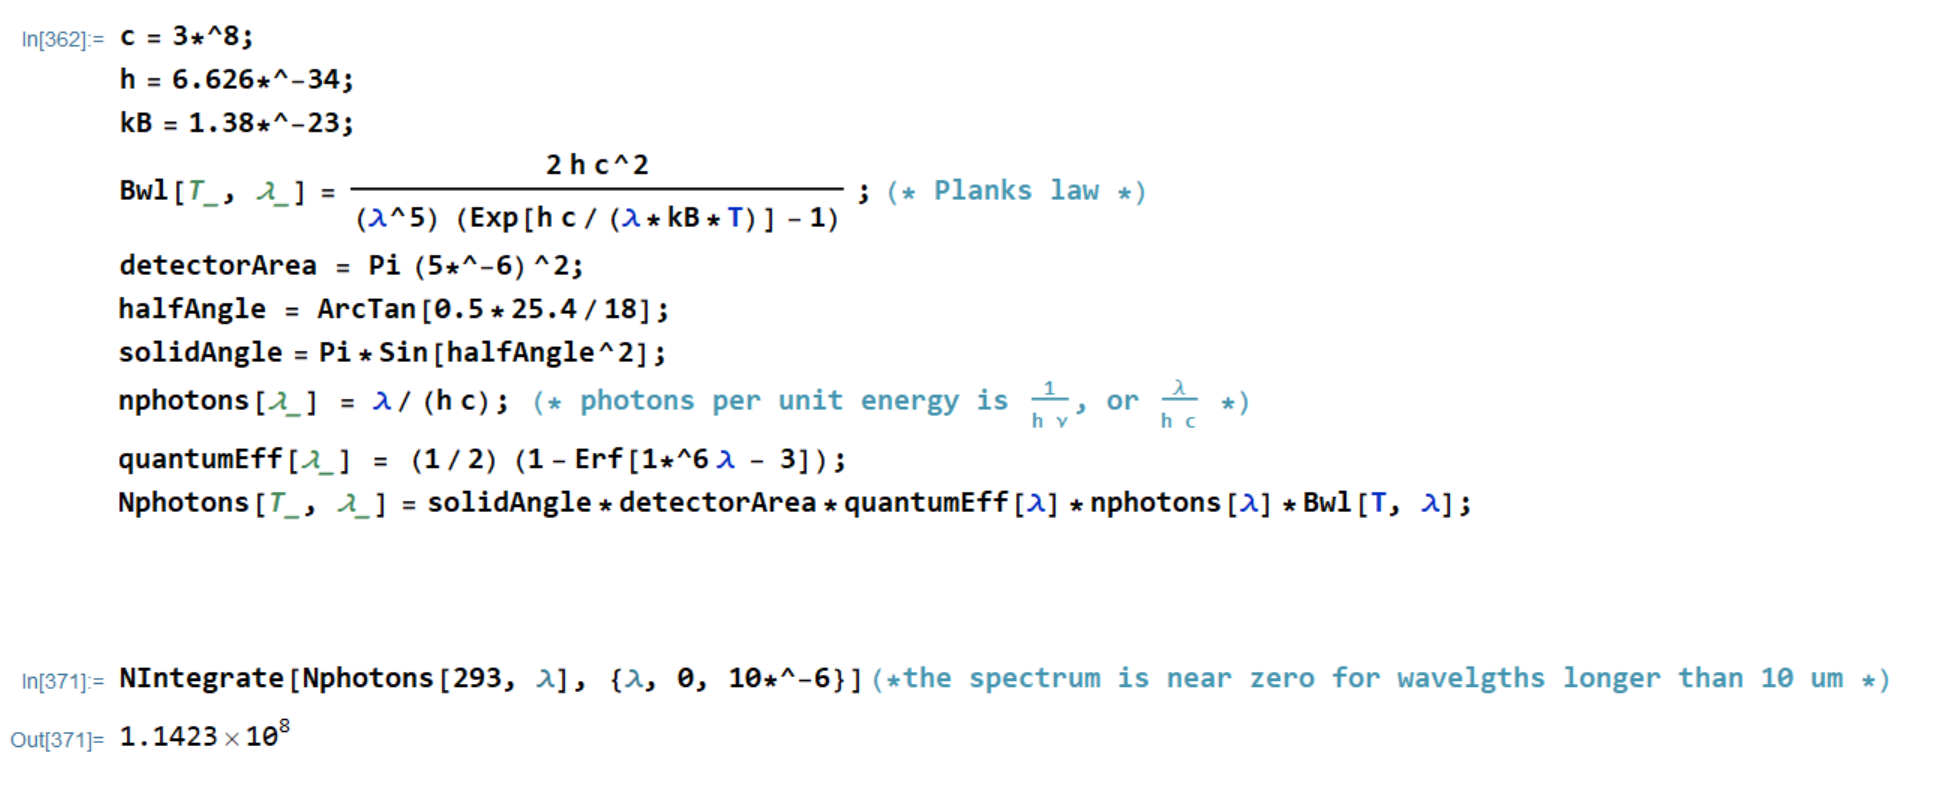
\includegraphics{chapter_05/figs_05/mathematica_2.PNG}}

  \textcolor{midnightblue}{Dark count rate
  \(\approx \boxed{110 \,\text{MCounts/s}}\) }
  \textcolor{midnightblue}{The rate of dark counts exceeds the usual
  maximum count rate, the detector is not usable. }

  \textcolor{midnightblue}{3 pts. for similar dark count rate (+/- 20\%)
  , 3 pts. for saying the detector is not usable.}
\item
  (6 pts) A set of shortpass filters can remove the bulk of blackbody
  radiation. A shortpass filter can be roughly modeled with the formula:

  \[F(\lambda, E_t) = \frac{1}{E_t}[(E_t - 1)H(\lambda_c - \lambda) + 1]\]

  Where H is the Heaviside step function, \(\lambda_c\) is the cutoff
  wavelength of the filter, and \(E_t\) is the extinction ratio of the
  filter. Use this with \(N_{photons}[\lambda]\) from (d). How many
  filters with \(\lambda_c = 1560~\text{nm}\) and \(E_t = 30~\text{dB}\)
  are necessary to suppress the spectral region of detectable dark
  counts longer than 1560 nm so that it is not the dominant source of
  dark counts?

  \textcolor{midnightblue}{ \textbf{Answer:} }

  \textcolor{midnightblue}{\(\boxed{\text{3 filters}}\) are needed to
  make the wavelength band shorter than 156 nm the dominant source of
  counts.} {3 pts. for this answer}

  \textcolor{darkred}{3 pts for evidence:}
  \textcolor{midnightblue}{Students might integrate the detectable dark
  count spectrum with different numbers of filters and comparing the
  results. The computations below show the addition of a fourth filter
  has a negligible effect on the dark count rate. }

  \textcolor{midnightblue}{Students may instead give a more qualitative
  answer, for example with a graph of the filtered spectrums, that shows
  the relative suppression of the region longer than 1560 nm. }

  \textcolor{midnightblue}{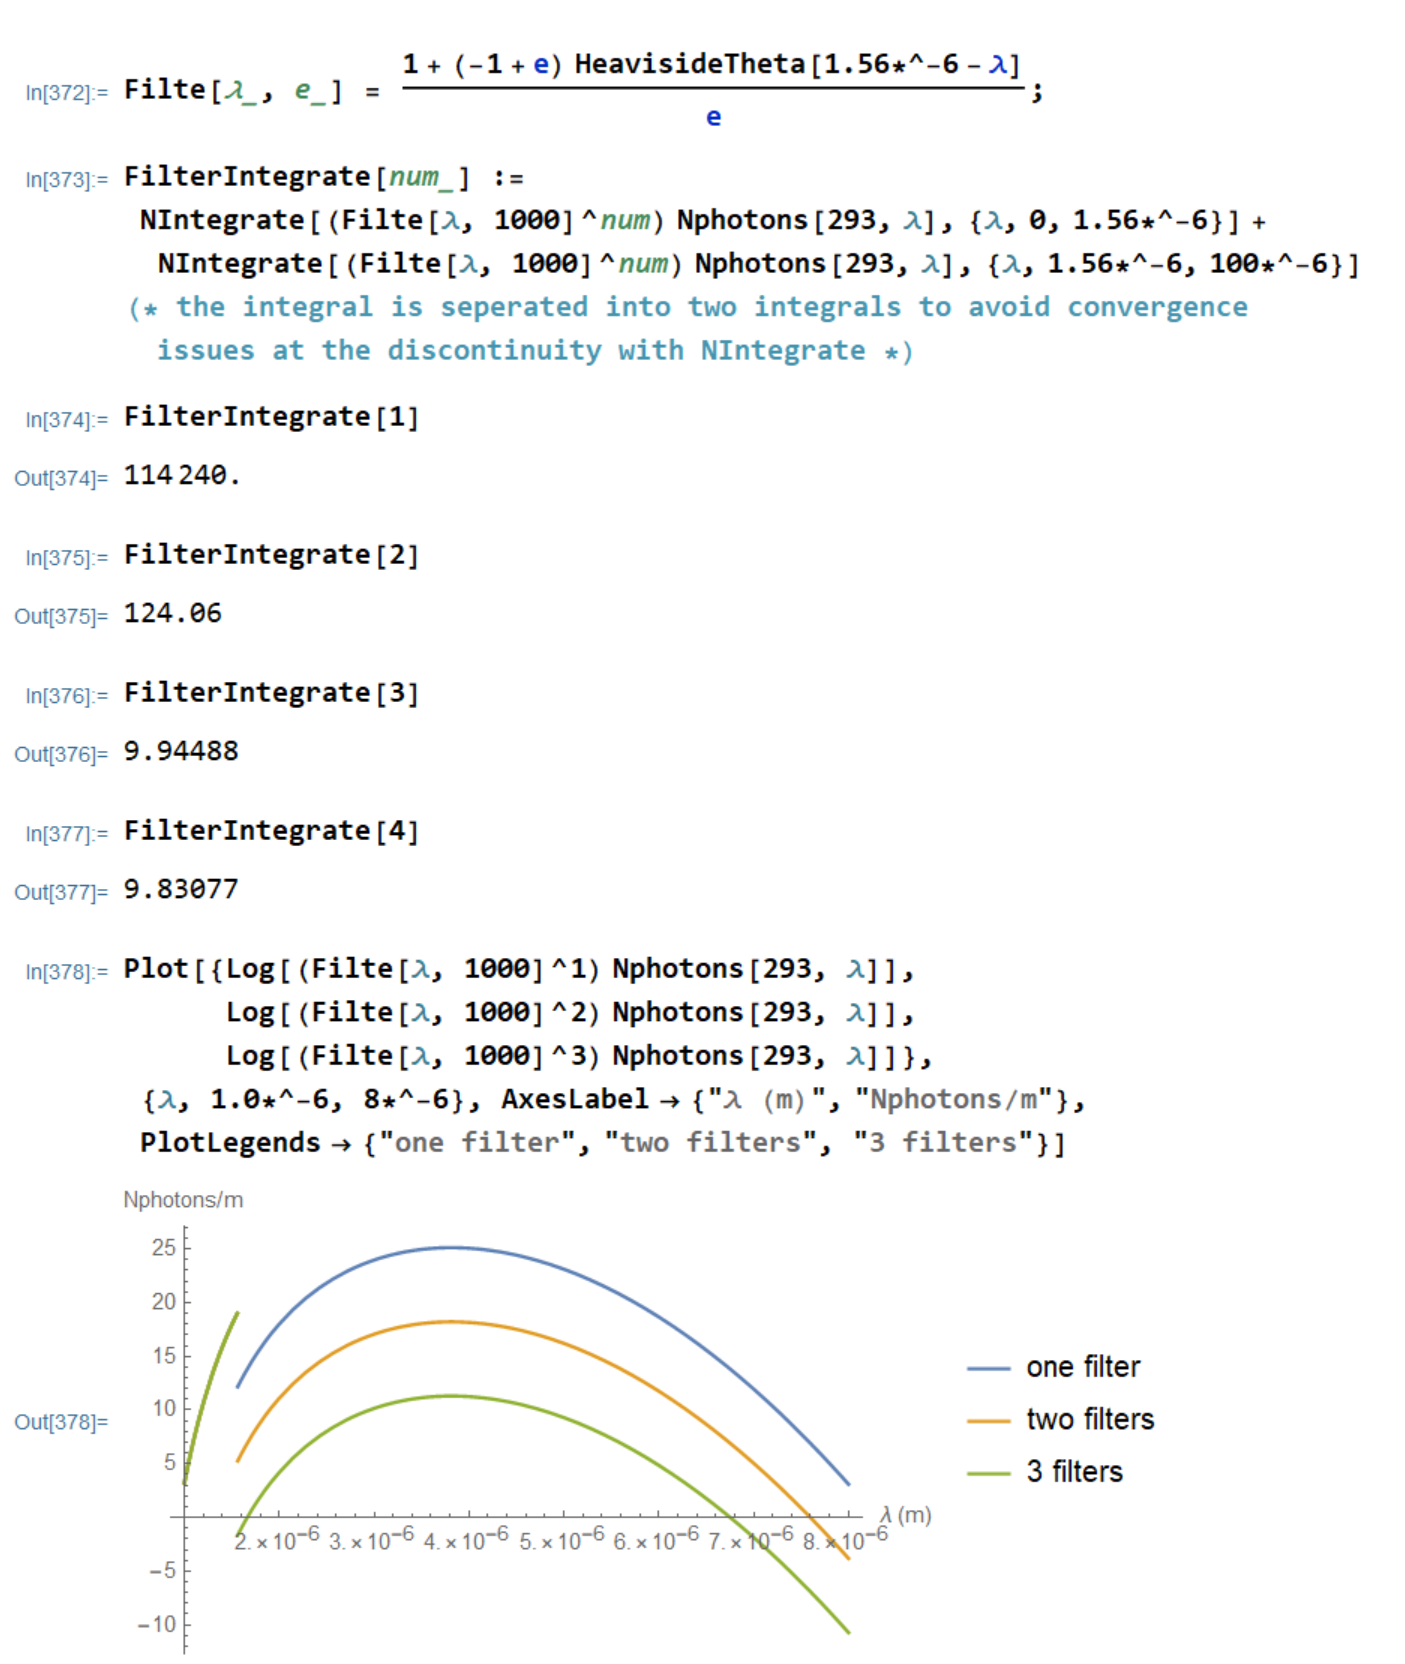
\includegraphics{chapter_05/figs_05/filter_integrate_4.PNG}}
\item
  (7 pts) If a narrow band filter is also inserted with center
  wavelength \(1550~\text{nm}\) and spectral width below \(1-2~nm\),
  then dark count rate can be approximated as just
  \(N_{photons}[\lambda = 1550~\text{nm}]\) times the filter width. Show
  for this wavelength range you can simplify dark count rate further to
  a simple exponential function. If the laboratory air conditioner
  breaks, raising the lab temperature from 293 K to 300 K, how much
  higher is the dark count rate?

  \textcolor{midnightblue}{ \textbf{Answer:} }

  \textcolor{midnightblue}{The expression for \(N_{photons}[\lambda]\)
  from part (1.4) can be simplified and evaluated at 1550 nm, then
  multiplied by the filter width in nanometers. }

  \textcolor{midnightblue}{

  \[\begin{aligned}
   N_{photons}[\lambda] &= P \Omega D_{area} \eta(\lambda) B_{\lambda}(\lambda) \\
   N_{filter} &= N_{photons}[\lambda = 1550~\text{nm}]\Delta \lambda
   \end{aligned}\]

  }

  \textcolor{midnightblue}{This code shows integrating the spectrum and
  just multiplying \(N_{photons}\) times the filter width produce very
  similar results (for a 1 nm filter):}

  \textcolor{midnightblue}{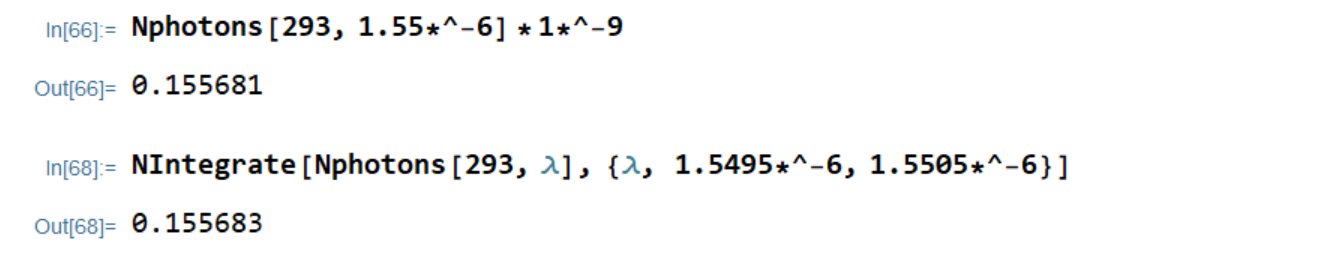
\includegraphics{chapter_05/figs_05/nphoton_approx.PNG}}

  \textcolor{midnightblue}{Evaluating the \(N_{photon}\) function at
  \(\lambda = 1550~text{nm}\) shows the \(-1\) term is small relative to
  the exponential term:}

  \textcolor{midnightblue}{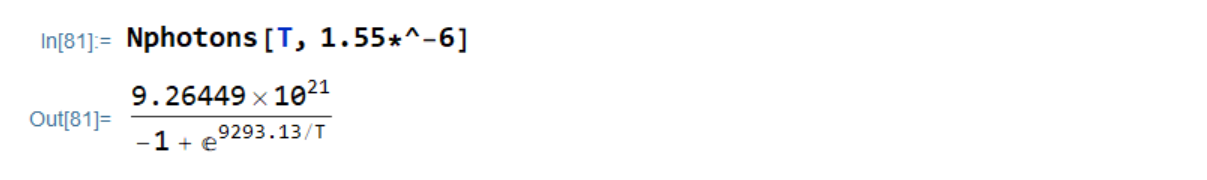
\includegraphics{chapter_05/figs_05/small_relative_to_exponential.PNG}}

  \textcolor{midnightblue}{Therefore the filter transmission
  approximation is:}

  \textcolor{midnightblue}{

  \[\boxed{N_{filter} \approx 9.26\mathrm{e}21 \Delta\lambda e^{-9290/T} (\frac{\text{photons}}{\text{s*meter}})}\]

  }

  \textcolor{midnightblue}{or equivalently: }

  \textcolor{midnightblue}{

  \[\boxed{N_{filter} \approx 9.26\mathrm{e}12 \Delta\lambda e^{-9290/T} (\frac{\text{photons}}{\text{s*nm}})}\]

  }

  \textcolor{midnightblue}{and the dark count rate in the 300 K room is
  roughly double the rate in the 293 K room: }

  \textcolor{midnightblue}{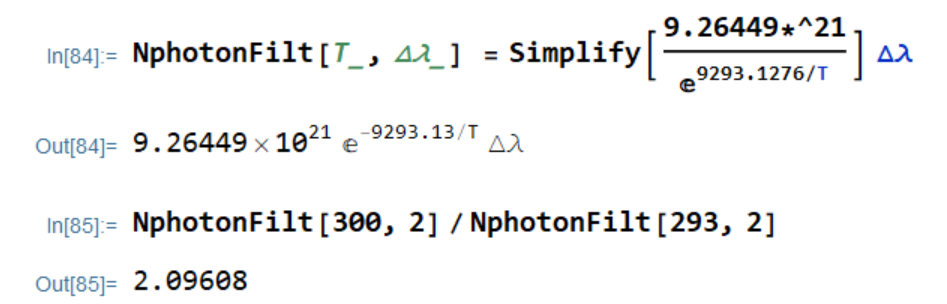
\includegraphics{chapter_05/figs_05/filter_with_temp.PNG}}

  \textcolor{midnightblue}{4 pts for a similar equation, 3 pts for
  finding the dark count rate roughly doubles. }

  A quantum communication experiment requires time-tagging photons with
  respect to a 50 GHz clock with 95\% fidelity. That is, 95\% of the
  timing measurements of detected photons emitted at the same time with
  respect to a clock fall within a 20 ps bin. Say the detector and
  readout electronics have a combined jitter of 10 ps FWHM, and a mode
  locked laser is used for the experiment that generates
  transform-limited Gaussian pulses. You tune it's temporal length to a
  value for which the total timing uncertainty of time-tagged photons
  --- including system jitter and pulse temporal length --- matches the
  95 \% fidelity at 50 GHz requirement. Assume detector jitter has a
  Gaussian shape as well.
\item
  (8 pts) Find the spectral width of a filter that would transmit 95\%
  of the photons from the mode locked laser. What is the dark count rate
  with this filter, using the expression from (1.7) and T = 293 K?

  \textcolor{midnightblue}{ \textbf{Answer:} }

  \textcolor{midnightblue}{For transform limited guassian pulses, the
  product of temporal and spectral width at a FWHM level is
  \href{https://www.lasercalculator.com/transform-limited-pulse-calculator/}{about
  0.441}. There's a derivation of this
  \href{https://www.physicsforums.com/threads/time-bandwidth-product-ideal-mode-locking.171404/post-1339948}{here},
  but students don't need to show it. }

  \textcolor{midnightblue}{

  \[T B P_{\text {Gaussian }}=\frac{2 \log 2}{\pi} \approx 0.441\]

  }

  \textcolor{midnightblue}{ Since this uses the FWHM level, all the 95\%
  metrics need to be converted. About 95\% of the area under a guassian
  falls within \(\pm 2 \sigma\). }

  \textcolor{midnightblue}{ Bound on total system timing uncertainty:
  \(20~\text{ps}_{95\%} = (20/4)*2.35 = 11.75~\text{ps}_{FWHM}\) }

  \textcolor{midnightblue}{ The jitter of the detection system and the
  temporal width of the laser pulse \(\Delta t\) should add in
  quadrature to match the bound: }

  \textcolor{midnightblue}{

  \[ 11.75~\text{ps}_{FWHM} = \sqrt{ \Delta t^2 + (10~\text{ps})^2}\]

  }

  \textcolor{midnightblue}{

  \[ 0.441 = \Delta t \Delta \nu \] \[\Delta \nu = 71~\text{GHz}\]
  \[\Delta \lambda = \frac{\lambda^2 \Delta \nu}{c} = 0.57~\text{nm}\]

  }

  \textcolor{midnightblue}{ \(0.57~\text{nm}\) is the spectral width of
  the laser pulse at the FWHM level. If this pulse passes through a
  tophat filter with width equal to the 95\% level of the laser pulse,
  then 95\% will be transmitted. }

  \textcolor{midnightblue}{Filter width: }

  \textcolor{midnightblue}{

  \[\Delta \lambda_{95\%} = \frac{4 \Delta \lambda}{2.35} \approx \boxed{1~\text{nm}} \]

  }

  \textcolor{midnightblue}{Dark count rate is easy to find using the
  expression from the previous section: }

  \textcolor{midnightblue}{

  \[\boxed{N_{filter} \approx 9.26e12 (1~\text{nm}) e^{-9290/T} (\frac{\text{photons}}{\text{s*nm}})} \approx 0.15~\text{photons/s} \]

  }

  \textcolor{midnightblue}{3 points for writing and solving the equation
  that matches the jitter bound to the quadrature sum }
  \textcolor{midnightblue}{5 points for correct filter width and dark
  count rate}
\end{enumerate}

\hypertarget{spdc-coupling-and-single-photon-sources-50-points}{%
\subsection{2. SPDC Coupling and Single Photon Sources (50
points)}\label{spdc-coupling-and-single-photon-sources-50-points}}

A Spontaneous Parametric Down Conversion (SPDC) crystal is known to
generate a twin beam squeezed state of the form:

\[|\psi\rangle= \sqrt{1 - \gamma^2} \sum_{n=0}^{\infty} \gamma^{n}\left|n_{s}, n_{i}\right\rangle \]

Where \(n_s\) and \(n_i\) are the number of photons corresponding to the
signal and idler parts of the wavefunction. Consider Fig.~\ref{fig:hsps}
a, where the crystal is pumped with a pulsed laser, and the the signal
and idler components that emerge are separated either by polarization or
frequency. The idler arm is sent to an SNSPD. This configuration can be
used as a heralded single photon source (HSPS). A click on the detector
on the idler arm `heralds' a non-vacuum state in the signal arm. High
fidelity and probability single photon sources are very useful for
various quantum optics experiments and technologies, including linear
optical quantum computing.

\hypertarget{fig:hsps}{%
\begin{figure}
\centering
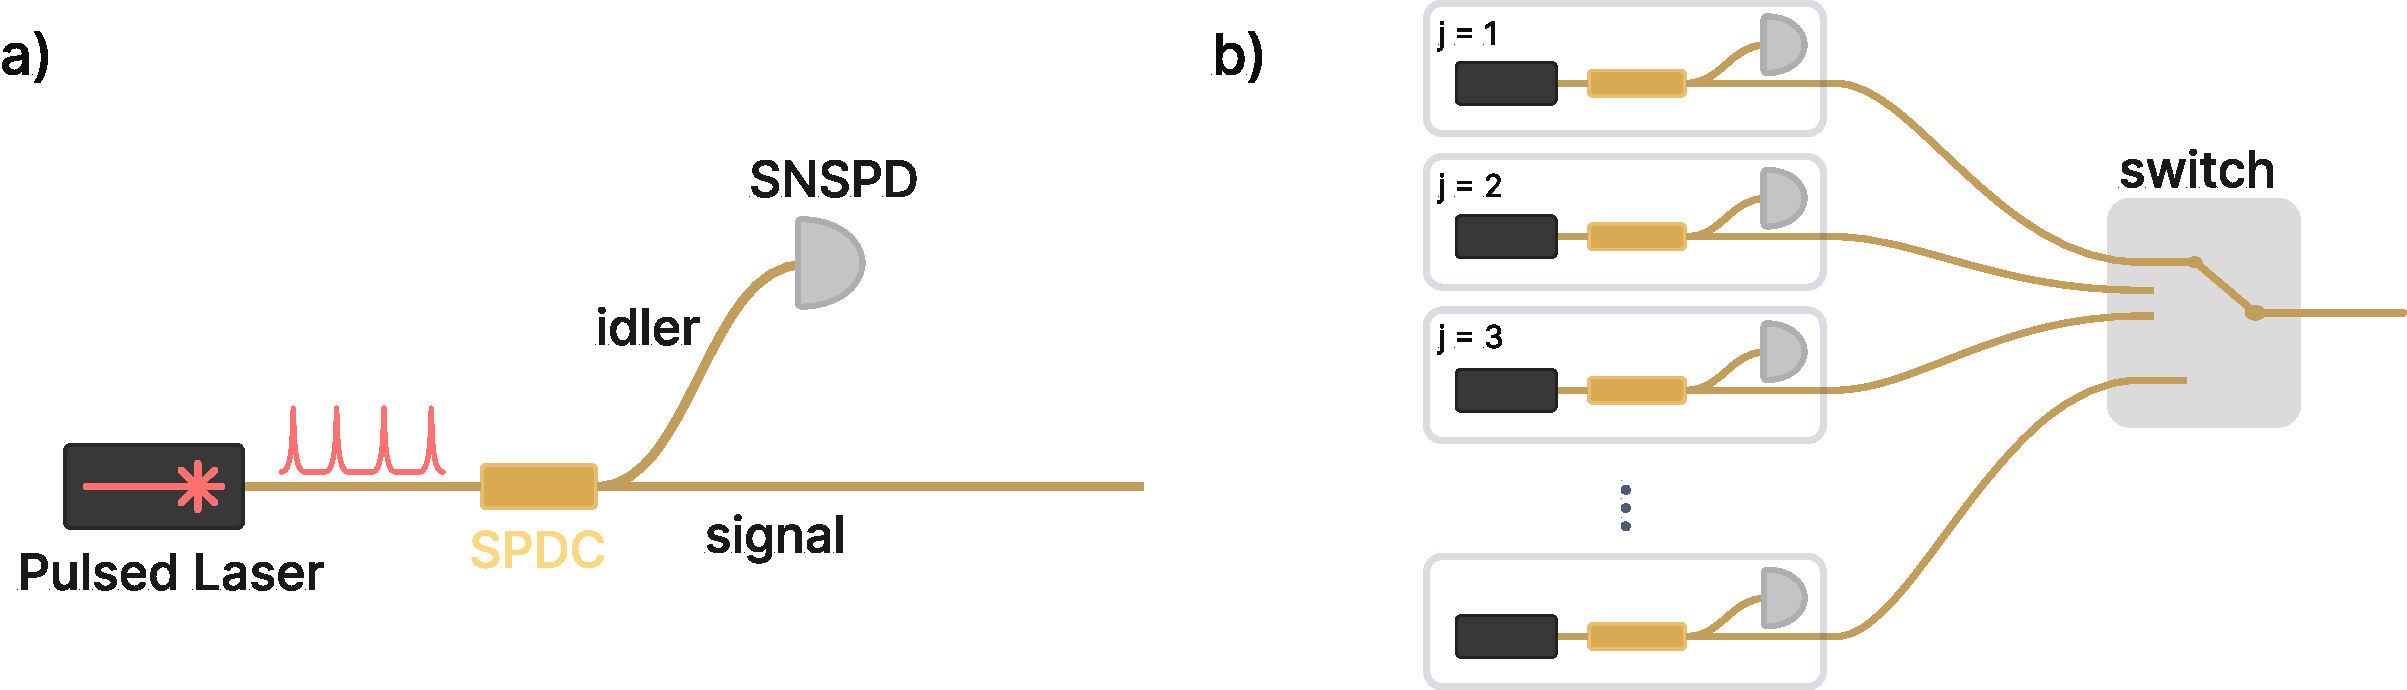
\includegraphics{chapter_05/figs_05/hsps_light.pdf}
\caption[{Heralded single photon source designs}]{\textbf{Heralded
single photon sources}}
\label{fig:hsps}
\end{figure}
}

Most SNSPDs are \emph{binary}-type single photon detectors, meaning they
differentiate between zero and one or more photons arriving in a given
light pulse. A positive operator value measure (POVM) quantifies how a
`click' from a binary SPD updates our knowledge of the incident state:

\[\hat{\Pi}_{\text {binary}} = \sum_{n=0}^{\infty}\left[1-(1-\eta)^{n}\right]|n\rangle\langle n|\]

Where \(\eta\) is the coupling efficiency between the state of interest
and the detector.

\begin{enumerate}
\def\labelenumi{\arabic{enumi}.}
\item
  (6 pts) Find the expectation value of \(\hat{\Pi}_{\text {binary}}\)
  given the SPDC state above. This is the probability
  \(p_{binary}\left(\gamma, \eta\right)\) of getting a binary detector
  click on the idler arm. For \(\gamma << 1\), what is \(p_{binary}\) up
  to lowest order in \(\gamma\), and what fock state of the signal arm
  is the source of this dominant term?

  \textcolor{midnightblue}{ \textbf{Answer:} }

  \textcolor{midnightblue}{

  \[\begin{aligned}
   \langle \psi | \Pi_{\text {binary}} | \psi \rangle &= (1- \gamma^2) \sum_{\tilde{n}=0}^{\infty} \langle \tilde{n}_s \tilde{n}_i | \gamma^{\tilde{n}} \sum_{n=0}^{\infty}[1 - (1-\eta)^{n}] \gamma^n | n_s n_i \rangle \\
   \langle \psi | \Pi_{\text {binary}} | \psi \rangle &= p_{binary}(\gamma, \eta) =  \boxed{(1-\gamma^2) \sum_{n_s=0}^{\infty} \gamma^{2n_s} [1 - (1 - \eta)^{n_s}]}
   \end{aligned}\]

  }

  \textcolor{midnightblue}{For
  \(\gamma << 1, ~~ p \sim (1 - \gamma^2)[\cancel{\gamma^0[1 - (1 - \eta)^0]} + \gamma^{2}\eta ] \sim (1 - \gamma^2)\gamma^{2}\eta\)
  }

  \textcolor{midnightblue}{ To lowest order in \(\gamma\),
  \(p \sim \gamma^{2}\eta\). The single photon fock state dominates for
  \(\gamma << 1\). }

  \textcolor{midnightblue}{ 3 pts for correct
  \(p_{binary}(\gamma, \eta)\); 3 pts for saying the leading term is
  from single photons }
\item
  (6 pts) A general form for the density matrix of the signal mode given
  a herald event is:

  \[\rho_{s}\left(\gamma, \eta\right)=\frac{\operatorname{Tr}_{i}\left(\hat{\Pi}|\psi\rangle\langle\psi|\right)}{\left\langle\psi\left|\hat{\Pi}\right| \psi\right\rangle}\]

  Write down the \(|1\rangle\langle1|\) term of this matrix, and
  simplify any infinite sums. This is the single photon fidelity
  \(F_{binary}(\gamma, \eta)\). Why does \(F_{binary}\) approach zero
  for \(\gamma\) approaching 1? What types of states is the SPDC
  generating in this limit?

  \textcolor{midnightblue}{ \textbf{Answer:} }

  \textcolor{midnightblue}{

  \[\begin{aligned}
   \rho_s(\gamma,\eta) &= \frac{\operatorname{Tr}_i[\cancel{(1 - \gamma^2)}\Sigma_{n=0}^{\infty} \gamma^{2n}[1 - (1 - \eta)^{n} ]| n \rangle \langle n | n_s n_i \rangle \langle n_s n_i |]}
   {\cancel{(1-\gamma^2)} \sum_{n_s=0}^{\infty} \gamma^{2n_s} [1 - (1 - \eta)^{n_s}]}\\
   |1_s \rangle \langle 1_s | &= \frac{\gamma^2[1 - (1 - \eta)]}{\sum_{n_s=0}^{\infty} \gamma^{2n_s} [1 - (1 - \eta)^{n_s}]} = \frac{\gamma^2 \eta}{\sum_{n_s=0}^{\infty} \gamma^{2n_s} [1 - (1 - \eta)^{n_s}]}\\
   |1_s \rangle \langle 1_s | &= \frac{\gamma^2 \eta}{\sum_{n_s=0}^{\infty}(\gamma^{2n_s} - [\gamma^2 (1 - \eta)]^{n_s})}\\
   &= \frac{\gamma^2 \eta}{\frac{1}{1 - \gamma^2} - \frac{1}{1 - \gamma^2(1 - \eta)}}\\
   &= \frac{\gamma^2 \eta (1 - \gamma^2)}{1 - \frac{1 - \gamma^2}{1 - \gamma^2(1 - \eta)}}\\
   &= \frac{\cancel{\gamma^2 \eta} (1 - \gamma^2) (1 - \gamma^2 (1 - \eta))}{\cancel{1 - \gamma^2 (1 - \eta) - 1 + \gamma^2}} \\
   F_{binary}(\gamma, \eta) &= \boxed{(1 - \gamma^2)(1 - \gamma^2(1 - \eta))}
   \end{aligned}\]

  }

  \textcolor{midnightblue}{As \(\gamma\) approaches 1, the denominator
  in the original expression for \(\rho_s(\gamma,\eta)\) approaches
  infinity while the numerator approaches \(\eta\). In this limit, the
  SPDC is generating predominantly multi-photon states. For \(\gamma\)
  approaching 1, the probability of the generated state being a single
  photon state goes to zero. Because the binary POVM was used,
  multi-photon states are `included' in \(\rho_s(\gamma,\eta)\). For
  \(\rho_s\) from the PNR POVM shown below, multi-photon states will be
  included to a much lesser extent, depending on the value for
  \(\eta\).}

  \textcolor{midnightblue}{3 pts for correct
  \(F_{binary}(\gamma, \eta)\); 3 pts for similar explanation}

  An HSPS with high single photon fidelity and probability is most
  useful, but you see these metrics are maximized for opposite limits of
  \(\gamma\). One approach to achieving high probability and fidelity
  simultaneously is to link multiple SPDC sources and heralding
  detectors as shown in Fig.~\ref{fig:hsps} b. A click from the detector
  \(j\) triggers the switch to move to position \(j\) and let the
  heralded state pass through. This way, \(\gamma\) for each source can
  be kept low to maximize fidelity, while heralding probability
  increases with the number of sources.
\item
  (6 pts) If such a multiplexing setup is engineered to have 98\% single
  photon fidelity from each source and 98\% heralding probability
  overall, how many sources and binary SNSPDs are needed? Use an idler
  arm efficiency \(\eta\) of 80\%.

  \textcolor{midnightblue}{ \textbf{Answer:} }

  \textcolor{midnightblue}{The fist step is to determine the pump power
  \(\gamma\) for which fideltiy is 98\%. }

  \textcolor{midnightblue}{

  \[0.98 = F_{binary}(\gamma, \eta) = (1 - \gamma^2)(1 - \gamma^2(1 - \eta)\,\,\,\,\,\,\,\, \eta = 0.8\]

  }

  A numerical solution is fine. We're interested in the positive
  solution less than one:

  \textcolor{midnightblue}{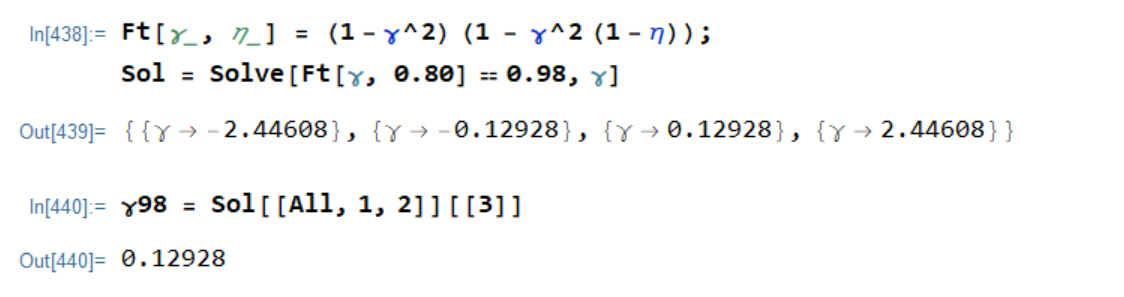
\includegraphics{chapter_05/figs_05/Ftsolve.PNG}}

  \textcolor{midnightblue}{Like in introductory statistics problems, its
  helpful to think about the negative case: Given N sources with herald
  probability \(p\), the probability of zero sources heralding is:}

  \textcolor{midnightblue}{

  \[P(\text{no herald}|N) = (1 - p_{binary}\left(\gamma, \eta\right))^N\]

  }

  \textcolor{midnightblue}{Then the probability of at least one herald
  is 1 minus the previous expression:}

  \textcolor{midnightblue}{

  \[P(\text{at least one herald}|N) = 1 - (1 - p_{binary}\left(\gamma, \eta\right))^N\]

  }

  \textcolor{midnightblue}{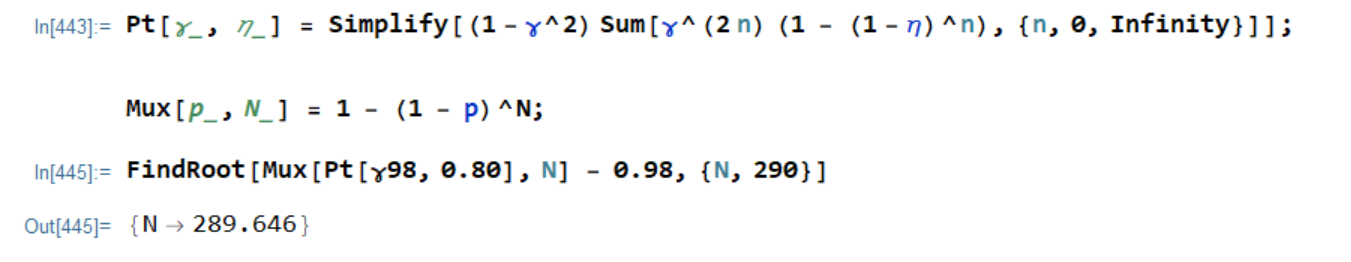
\includegraphics{chapter_05/figs_05/mux_binary.PNG}}

  \textcolor{midnightblue}{About \(\boxed{N = 290}\) sources are
  needed.}

  \textcolor{midnightblue}{3 pts for correct form of the multiplexing
  expression \(P(\text{at least one herald}|N)\); 3 pts for similar
  number of sources \(N\)}
\end{enumerate}

A photon number resolving (PNR) SNSPD is able to discriminate the number
of photons in a light pulse*. By heralding the idler mode with a PNR
SNSPD, the generation of multi-photon signal pulses can be identified
and discarded. There's a POVM for an ideal PNR single photon detector,
where \(i\) is the number of photons detected**:

\[\hat{\Pi}_{PNR}(i)=\sum_{n=i}^{\infty}\binom{n}{i}(1-\eta)^{n-i} \eta^{i}|n\rangle\langle n|\]

\begin{enumerate}
\def\labelenumi{\arabic{enumi}.}
\setcounter{enumi}{3}
\item
  (12 pts) Derive a herald probability \(p_{PNR}\) and fidelity
  \(F_{PNR}\) for the PNR POVM, following the steps in the previous
  sections with \(i\) set to 1. You can use symbolic math tools to
  simplify them if you wish. The probability of successfully heralding
  states in the signal arm \(p_{PNR}\) should now approach zero for
  \(\gamma\) near one. Why is this?

  \textcolor{midnightblue}{ \textbf{Answer:} }
  \textcolor{midnightblue}{The POVM for one photon detected:}

  \textcolor{midnightblue}{

  \[\hat{\Pi}_{PNR}(1)=\sum_{n=1}^{\infty}n(1-\eta)^{n-1} \eta|n\rangle\langle n|\]

  }

  \textcolor{midnightblue}{First, derive the probability of getting a
  single photon detection from the PNR detector:
  \(p_{PNR}(\gamma, \eta)\):}

  \textcolor{midnightblue}{

  \[\begin{aligned}
       p_{PNR}(\gamma, \eta) =\langle \psi | \Pi_{\text {PNR}} | \psi \rangle &= (1- \gamma^2) \sum_{\tilde{n}=0}^{\infty} \langle \tilde{n}_s \tilde{n}_i | \gamma^{\tilde{n}} \sum_{n=1}^{\infty}n(1-\eta)^{n-1} \eta|n\rangle\langle n| | n_s n_i \rangle \\
       \langle \psi | \Pi_{\text {PNR}} | \psi \rangle &= p_{PNR}\left(\gamma, \eta\right) =  \boxed{(1-\gamma^2) \sum_{n_s=0}^{\infty} \gamma^{2n_s} n_s(1-\eta)^{n_s-1}}\\
       p_{PNR}\left(\gamma, \eta\right) &=  \boxed{\frac{\gamma ^2 (1 - \gamma ^2) \eta }{(\gamma ^2 (\eta -1)+1)^2}}
   \end{aligned}\]

  }

  \textcolor{midnightblue}{Where either of the boxed answers are
  acceptable, and the last line was found using mathematica:}

  \textcolor{midnightblue}{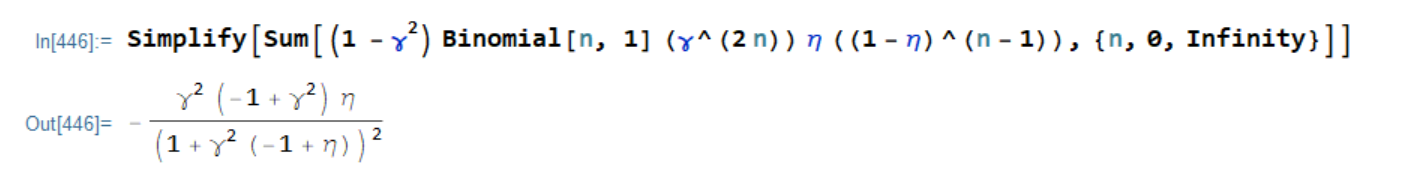
\includegraphics{chapter_05/figs_05/simplify_ppnr.PNG}}

  \textcolor{darkred}{4 pts for \(p_{PNR}\left(\gamma, \eta\right)\)}

  \textcolor{midnightblue}{Second, derive the single photon fidelity,
  staring with the density matrix for the signal photon given a PNR
  herald event. Using (15) above for
  \(\langle \psi | \Pi_{\text {PNR}} | \psi \rangle\) in the denominator
  helps simplify it significantly. }

  \textcolor{midnightblue}{

  \[\begin{aligned}
       \rho_s(\gamma,\eta) &= \frac{\operatorname{Tr}_i[\sum_{n=1}^{\infty} \gamma^{2n}n(1-\eta)^{n-1} \eta|n\rangle\langle n|n_s n_i \rangle \langle n_s n_i |]}
           {\langle \psi | \Pi_{\text {PNR}} | \psi \rangle}\\
           |1_s \rangle \langle 1_s | &= \frac{\cancel{(1 - \gamma^2)}(\gamma ^2 (\eta -1)+1)^2 \cancel{\gamma^2 \eta}}{\cancel{\gamma^2 \eta} \cancel{(1 - \gamma ^2)} }\\
           F_{PNR}(\gamma, \eta) &= \boxed{(\gamma ^2 (\eta -1)+1)^2}
   \end{aligned}\]

  }

  \textcolor{midnightblue}{4 pts for \(F_{PNR}(\gamma, \eta)\)}

  \textcolor{midnightblue}{For \(\gamma\) near one, the SPDC is under
  strong pump power and is generating predominantly multi-pair states. A
  vanishing fraction of those states are single photon states that the
  PNR detector is able to distinguish and single-photon. Therefore, the
  PNR detector is signaling the generation of multi-pair states most of
  the time which should be discarded and do not contribute to
  \(p_{PNR}\). For high efficiency \(\eta\), only the vanishing
  single-pair creation rate contributes predominantly to \(p_{PNR}\).}

  \textcolor{darkred}{4 pts for similar explanation}
\item
  (12 pts) Make a parametric plot for \(0<\gamma<1\) with \(F_{PNR}\) on
  the x-axis and \(p_{PNR}\) on the y-axis. Plot the curve for a few
  different values of idler arm efficiency \(0<\eta<1\). All curves
  should reach the same maximum herald probability. What is it?

  \textcolor{midnightblue}{ \textbf{Answer:} }
  \textcolor{midnightblue}{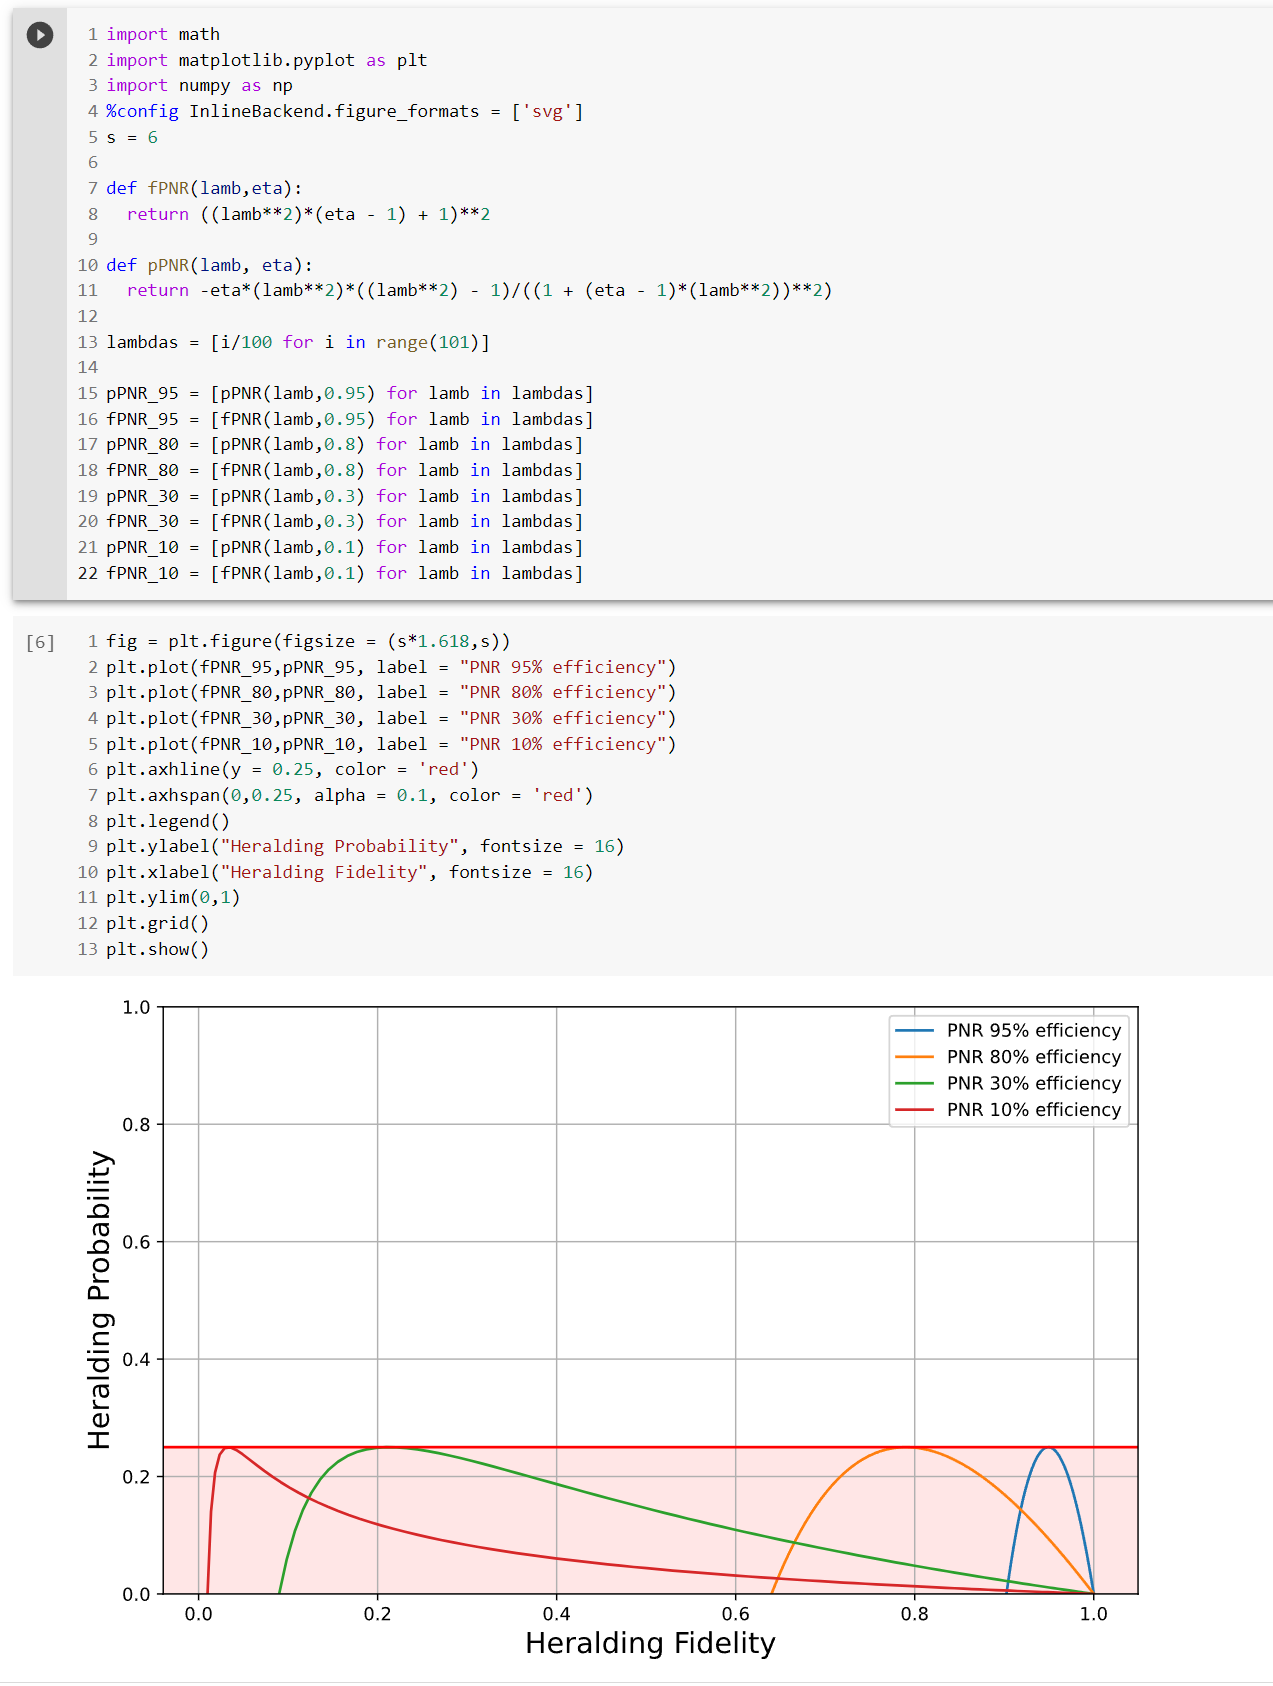
\includegraphics{chapter_05/figs_05/PLT.PNG}}

  \textcolor{midnightblue}{ The the herald probability regardless of
  idler arm efficiency is 25\%. }

  \textcolor{darkred}{ 4 points for the 25\% limit; 8 points for a few
  plots at different \(\eta\) }
\item
  (8 pts) Consider again the configuration in Fig.~\ref{fig:hsps} b.
  Find the number of sources using PNR detectors needed to reach 98\%
  single photon herald probability and fidelity with \(\eta = 0.8\).
  Also find the number of sources for \(\eta = 0.95\).

  \textcolor{midnightblue}{ \textbf{Answer:} }
  \textcolor{midnightblue}{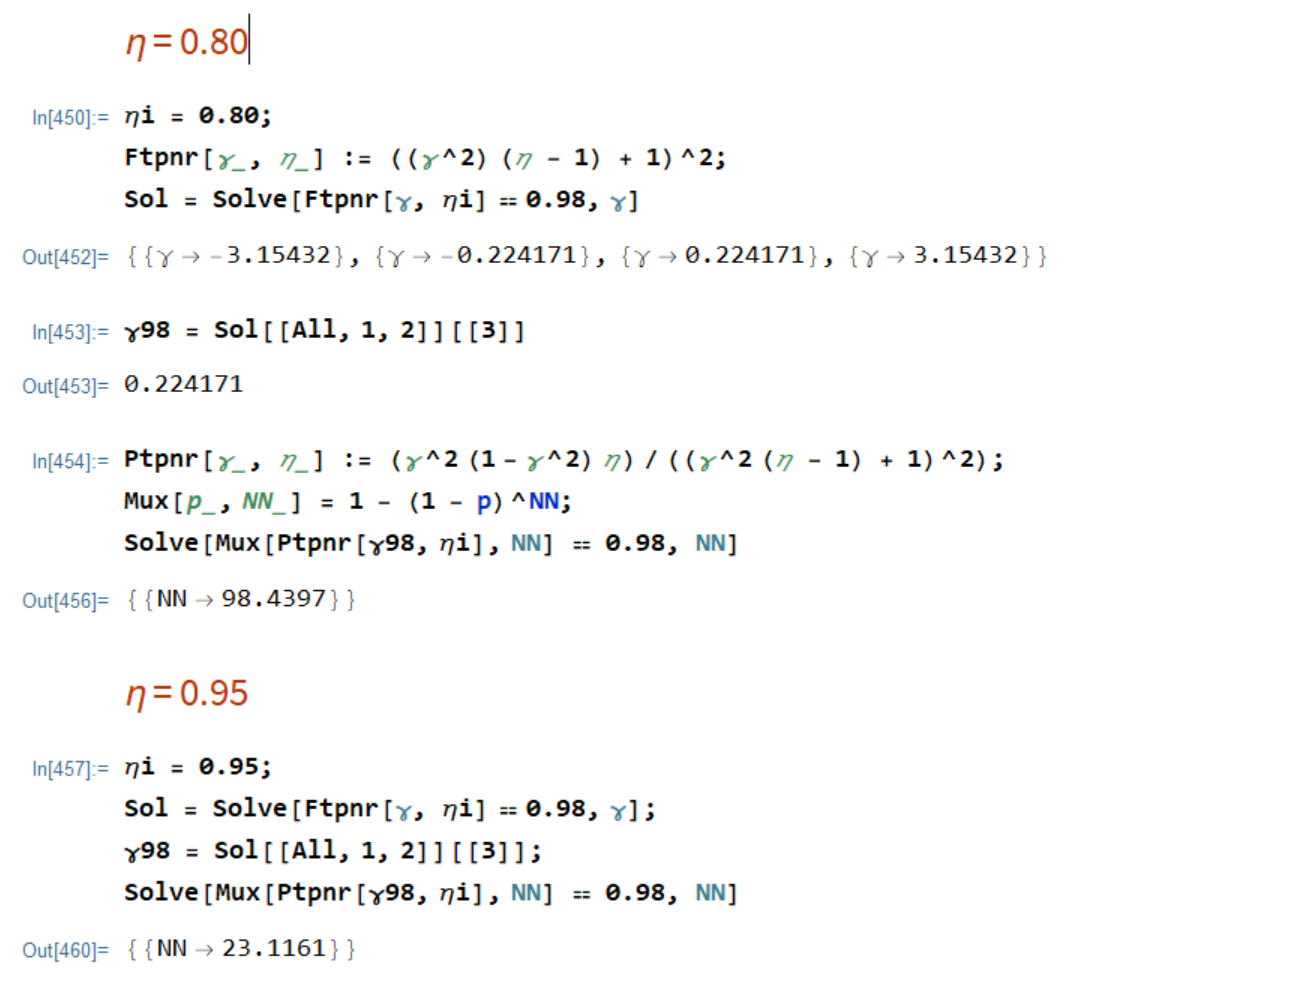
\includegraphics{chapter_05/figs_05/pnrTotalPerf.PNG}}

  \textcolor{midnightblue}{About
  \(\boxed{\text{98 sources are needed for the case with an 80\% heralding}}\),
  }

  \textcolor{midnightblue}{about
  \(\boxed{\text{23 sources are needed with 95\% efficient heralding}}\)}

  \textcolor{darkred}{ 4 points for each of the 2 answers. Answers that
  vary from these values by 2-3 sources are acceptable. }
\end{enumerate}

\hypertarget{aph-138-homework-assignment}{%
\chapter{Aph 138 Homework
Assignment}\label{aph-138-homework-assignment}}

\hypertarget{abstract-4}{%
\section{Abstract}\label{abstract-4}}

\hypertarget{software-systems-and-operation}{%
\section{Software Systems and
Operation}\label{software-systems-and-operation}}

\hypertarget{advanced-matplotlib-layouts-with-the-bisect-function}{%
\subsection{\texorpdfstring{Advanced Matplotlib Layouts with the
\texttt{bisect()}
function}{Advanced Matplotlib Layouts with the bisect() function}}\label{advanced-matplotlib-layouts-with-the-bisect-function}}

It can be difficult to create complex plot layouts with matplotlib,
especially when the layout should have strict requirements, like
neighboring axes that are aligned with one another. Before explaining a
custom method for solving this problem through the use of a new function
\texttt{bisect()}, its worth reviewing the more accepted methods of
advanced matplotlib figure layout.

\hypertarget{subplot-mosaic}{%
\subsubsection{Subplot Mosaic}\label{subplot-mosaic}}

\href{https://matplotlib.org/stable/gallery/subplots_axes_and_figures/mosaic.html}{Subplot
mosaic} is a tool for specifying the layout of a figure with a special
python dictionary, demonstrated by this example from the docs:

\begin{minted}
[
frame=lines,
framesep=2mm,
baselinestretch=1,
bgcolor=extralightgray,
fontsize=\footnotesize,
linenos]
{python}
fig = plt.figure(layout="constrained")
ax_dict = fig.subplot_mosaic(
    [
        ["bar", "plot"],
        ["hist", "image"],
    ],
)
ax_dict["bar"].bar(["a", "b", "c"], [5, 7, 9])
ax_dict["plot"].plot([1, 2, 3])
ax_dict["hist"].hist(hist_data)
ax_dict["image"].imshow([[1, 2], [2, 1]])
identify_axes(ax_dict)
\end{minted}

\includegraphics{chapter_05/figs_05/sphx_glr_mosaic_001_2_0x.webp}

There are methods of changing the aspect ratios of the plots, but tools
for imposing alignment constraints across plots are limited. For
example, notice in the example above how the (1,1) plot axes are not
vertically aligned with the (0,1) plot above.

\hypertarget{gridspec}{%
\subsubsection{Gridspec}\label{gridspec}}

\href{https://matplotlib.org/stable/gallery/lines_bars_and_markers/scatter_hist.html\#sphx-glr-gallery-lines-bars-and-markers-scatter-hist-py}{Gridspec}
is a tool for more carefully specifying a grid layout. Space between
plots can be specified, and the relative widths or heights of columns
and rows can be customized. Gridspec offers a lot of control, but it
requires many custom parameters that can be unintuitive to derive.

\hypertarget{add_axes}{%
\subsubsection{Add\_axes}\label{add_axes}}

One of the simplest ways of adding subplots to a figure is with the
\texttt{fig.add\_axese(rect)} method. The
\texttt{rect\ =\ {[}ll\_x,\ ll\_y,\ width,\ height{]}} specifies the x
and y coordinate of the lower left corner with the first two parameters,
and the width and height with the second 2 parameters. Multiple uses of
\texttt{add\_axese()} offers maximum control for creating advanced
layouts, but specifying all the correct \texttt{rect} arrays can get
very confusing. Figure Fig.~\ref{fig:layout_sketch} illustrates the
types of calculations that become necessary when the specific location
and size of each subplot must be specified under certain constraints.

\hypertarget{fig:layout_sketch}{%
\begin{figure}
\centering
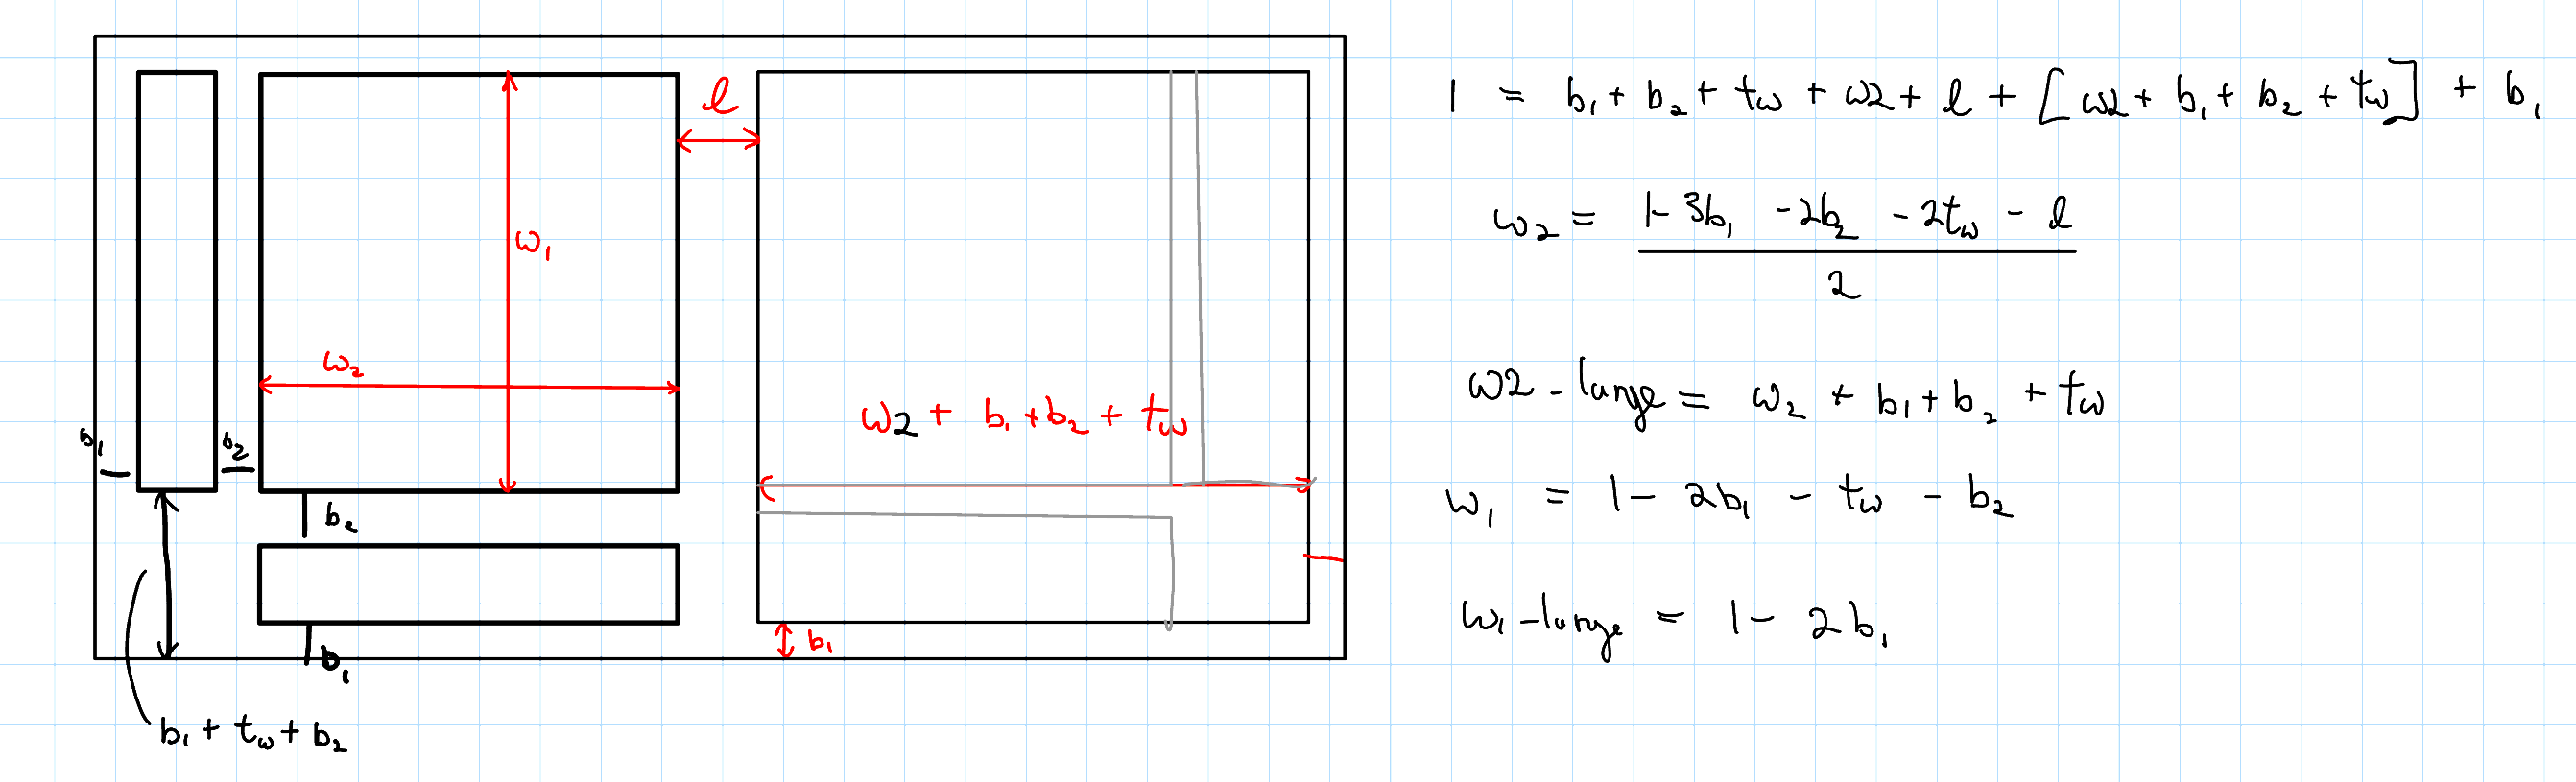
\includegraphics{chapter_05/figs_05/layout_sketch.png}
\caption[{Rough sketch for layout with add\_axese()}]{\textbf{Sketch for
layout with add\_axese().}}
\label{fig:layout_sketch}
\end{figure}
}

\hypertarget{bisect-method}{%
\subsubsection{\texorpdfstring{\texttt{bisect()}
method}{bisect() method}}\label{bisect-method}}

\hypertarget{how-a-sorption-fridge-works}{%
\section{How A Sorption Fridge
Works}\label{how-a-sorption-fridge-works}}

use \boldsymbol for bold latex:

\textbf{Fidelity and Rates vs \(\boldsymbol \mu\)}

Here are a few bold characters together:
\(\boldsymbol{\mu \quad \beta \quad \gamma}\)

For units, use \mathrm{nm}: This is a number with units:
\(138.3~\mathrm{nm}\)

Refer to a figure with Fig.~\ref{fig:figurename} or
Fig.~\ref{fig:figurename} or for multiple Fig.~\ref{fig:figurename}

Until I figure something more shorthand, you can set colors with
``\textless span\textgreater{}'' tags:

{\color{midnightblue}  This text is blue. And it changes lightness when
darkmode is witched }

\hypertarget{fig:figurename}{%
\begin{figure}
\centering
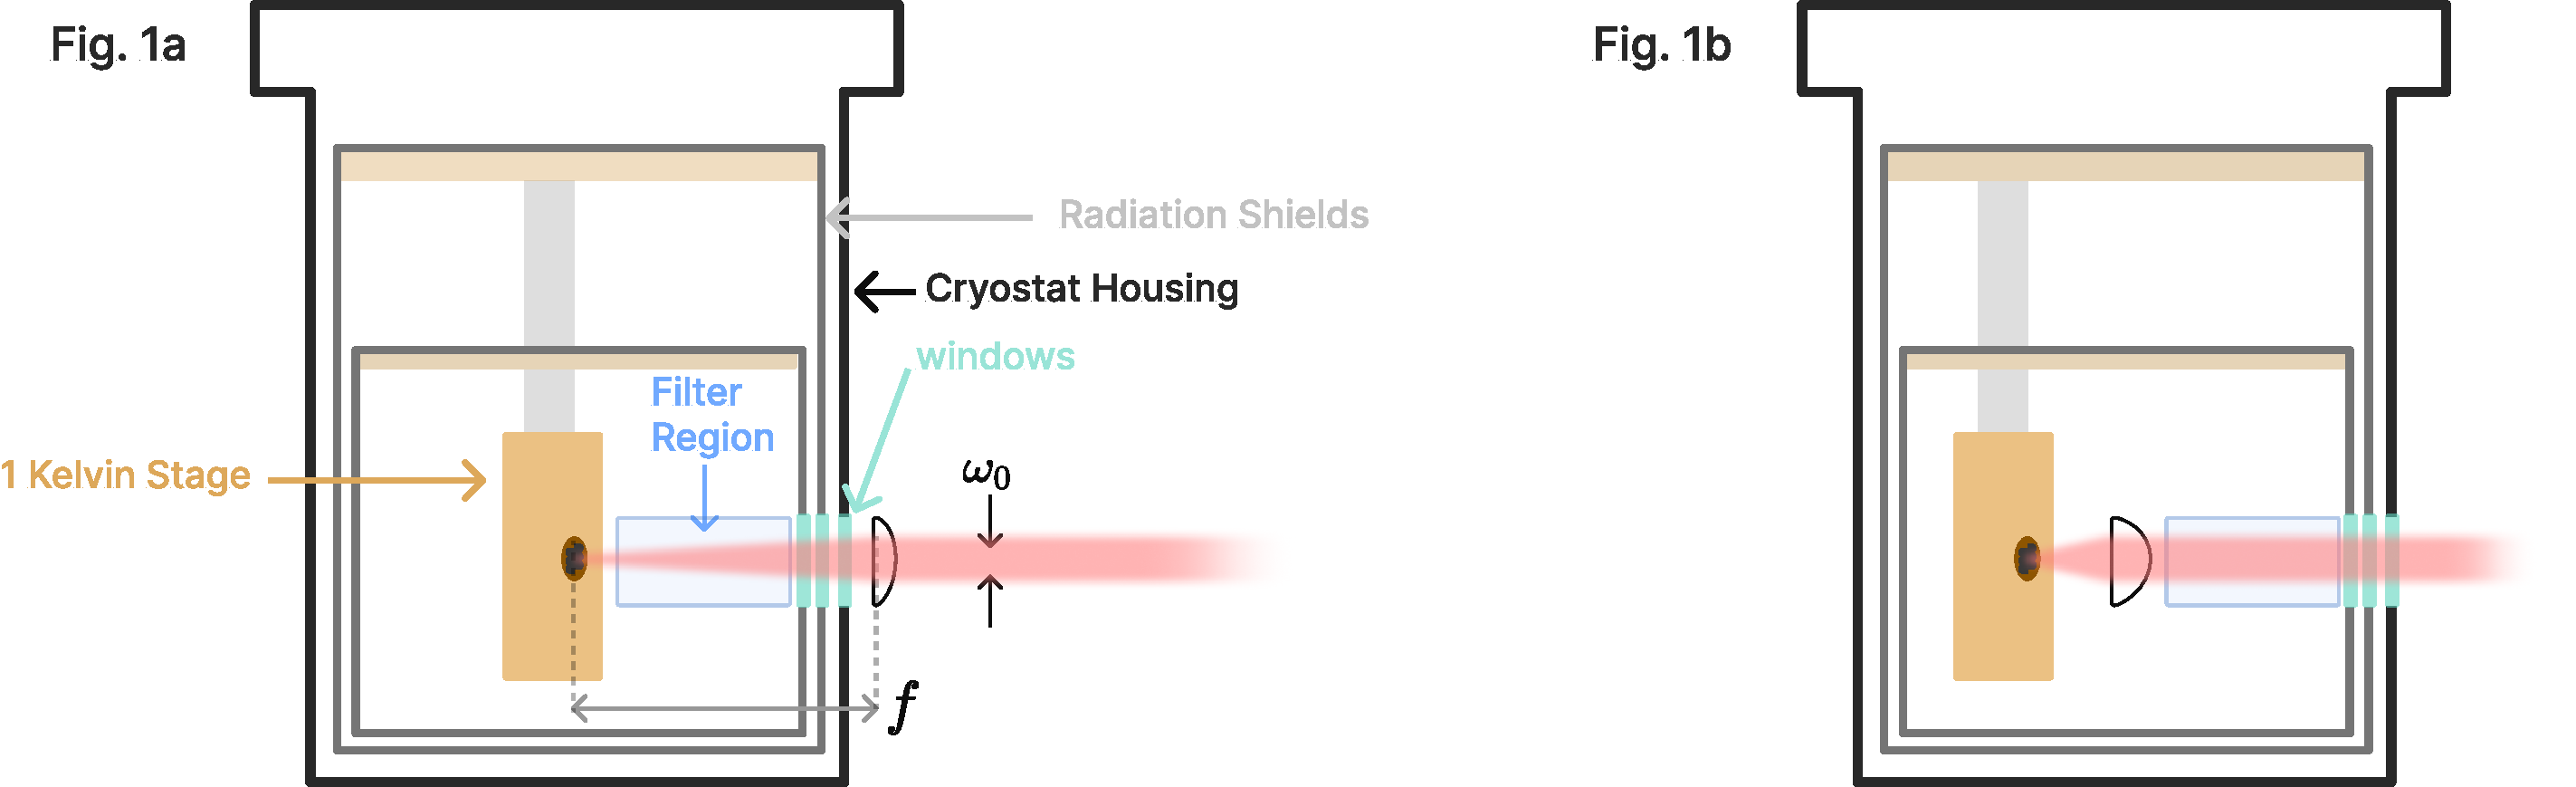
\includegraphics[width=0.7\textwidth,height=\textheight]{chapter_05/figs_05/fig1b_light.pdf}
\caption[{Figure label for in thesis index here.}]{\textbf{Caption title
here} a) Long caption here}
\label{fig:figurename}
\end{figure}
}

\hypertarget{fig:figurename2}{%
\begin{figure}
\centering
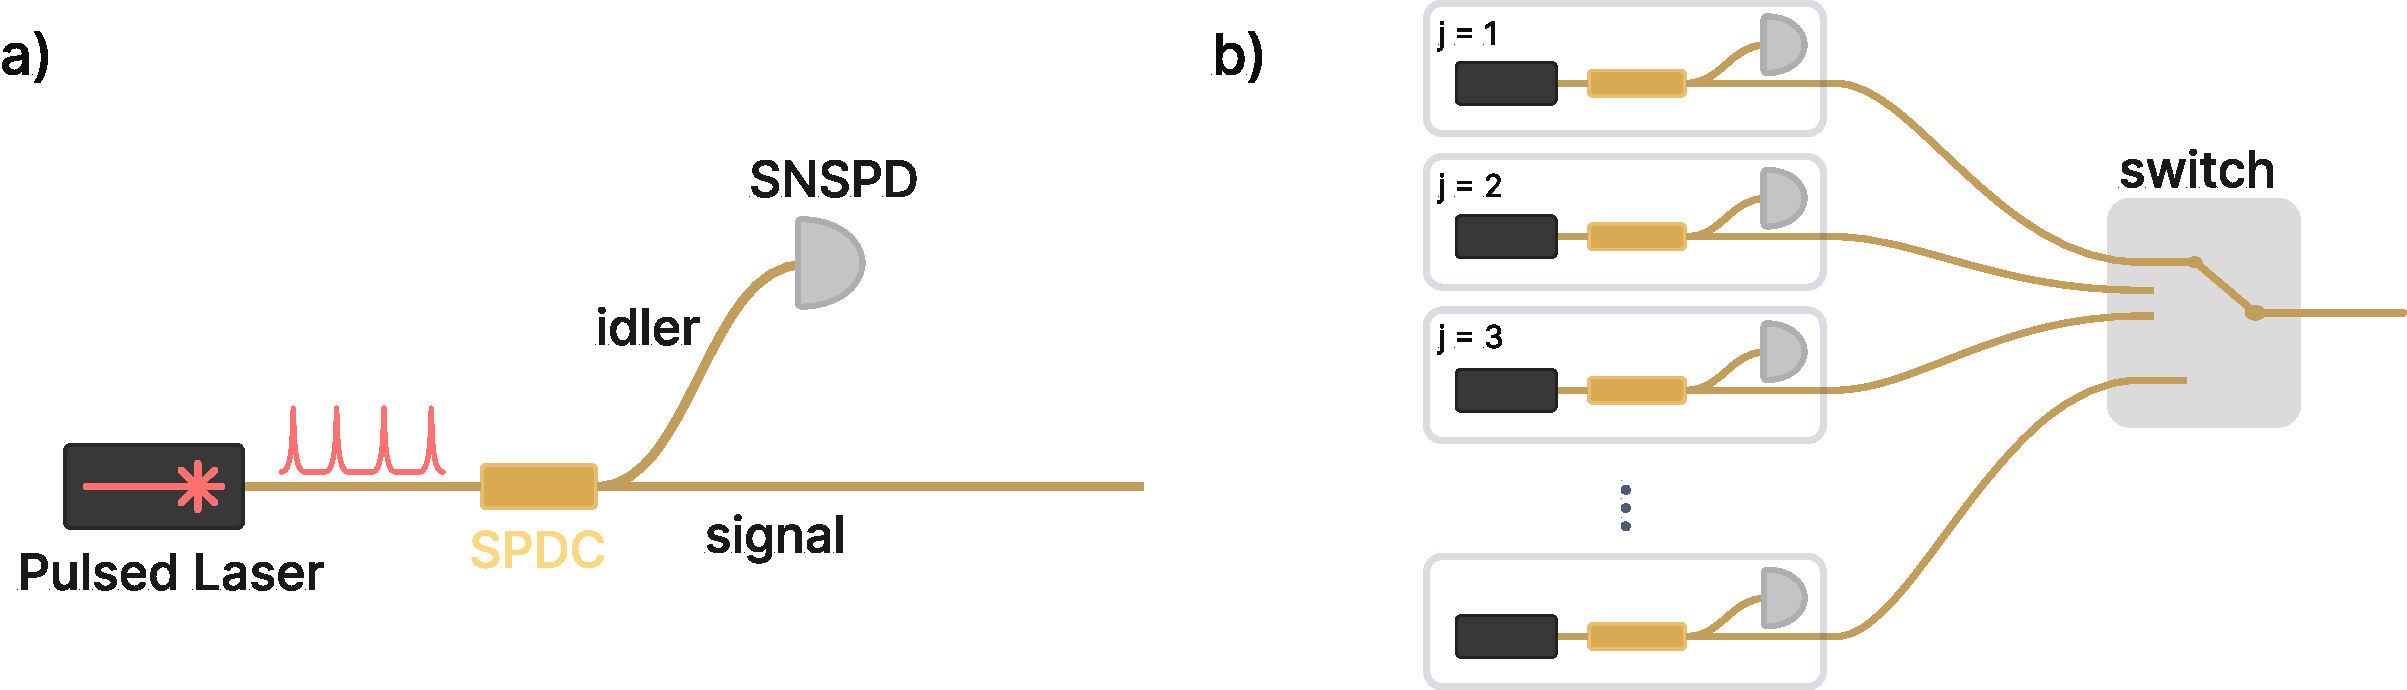
\includegraphics[width=0.7\textwidth,height=\textheight]{chapter_05/figs_05/hsps_light.pdf}
\caption[{Figure label for in thesis index here.}]{\textbf{Caption title
here} a) Long caption here}
\label{fig:figurename2}
\end{figure}
}

to have a ``\textasciitilde{}'' space in latex and a no break space in
html\ldots{} ``\&\#160'', just use ``~''. That's a forward slash and a
space.

The formatting of multi-line divs is very important. This will render
correctly:

{\color{midnightblue} 

\[math stuff 1\]

}

But this won't:

{\color{midnightblue} 

\begin{minted}
[
frame=lines,
framesep=2mm,
baselinestretch=1,
bgcolor=extralightgray,
fontsize=\footnotesize,
linenos]
{nil}
$$math stuff 2$$
\end{minted}

}

And this won't

\begin{minted}
[
frame=lines,
framesep=2mm,
baselinestretch=1,
bgcolor=extralightgray,
fontsize=\footnotesize,
linenos]
{nil}
$$math stuff 3$$

</div>
\end{minted}

the file where you're working on bokeh styling is at :

C:\Users\Andrew\OneDrive - California Institute of
Technology\JPL.Jitterate\peacoq\src\bokeh\_hists\_js\_callbacks.ipynb

\printbibliography
\end{document}
